\documentclass[spanish]{beamer}
%% \usetheme{Warsaw}
%% \usetheme{Madrid}

\usepackage[spanish]{babel}
\usetheme[beetle]{Boadilla}


 \useoutertheme{miniframes}
%% \useinnertheme{rounded}
%% \usecolortheme{}
\usepackage[utf8]{inputenc}
\usepackage{tikz}
\usepackage{wrapfig}
\usepackage{algorithmic, algorithm}
%% \usepackage{authblk}


%% \setbeameroption{show notes}


\usepackage{graphicx} 
%\usepackage{algorithmic}
%\usepackage{algorithm}
\newcommand{\formulasize}{\tiny}

\definecolor{rojo}{rgb}{0.7,0.1,0.1}
\definecolor{azul}{rgb}{0.1,0.1,0.7}
\definecolor{verde}{rgb}{0.1,0.4,0.1}

\newcommand{\rojo}[1]{\textcolor{rojo}{#1}}
\newcommand{\azul}[1]{\textcolor{azul}{#1}}
\newcommand{\verde}[1]{\textcolor{verde}{#1}}

%% \setcounter{secnumdepth}{5}

\newcommand{\Rojo}[1]{\textbf{\rojo{#1}}}
\newcommand{\Azul}[1]{\textbf{\azul{#1}}}
\newcommand{\Verde}[1]{\textbf{\verde{#1}}}

%%% Unified concepts commands

\newcommand{\opencl}{\emph{OpenCL}}

\newcommand{\pipeline}{\emph{pipeline}}
\newcommand{\Pipeline}{\emph{Pipeline}}

\newcommand{\wi}{\emph{work item}}
\newcommand{\wis}{\emph{work items}}
\newcommand{\wg}{\emph{work group}}
\newcommand{\wgs}{\emph{work groups}}

\newcommand{\Wi}{\emph{Work item}}
\newcommand{\Wis}{\emph{Work items}}
\newcommand{\Wg}{\emph{Work group}}
\newcommand{\Wgs}{\emph{Work groups}}

\newcommand{\bbox}{BBox}
\newcommand{\bboxes}{BBoxes}
\newcommand{\bvh}{BVH}
\newcommand{\bvhs}{BVHs}

\newcommand {\raytracer}{\emph{ray tracer}}
\newcommand {\raytracers}{\emph{ray tracers}}
\newcommand {\raytracing}{\emph{ray tracing}}
\newcommand {\Raytracer}{\emph{Ray tracer}}
\newcommand {\Raytracers}{\emph{Ray tracers}}
\newcommand {\Raytracing}{\emph{Ray tracing}}

%%% Style fix so institue doesnt appear on brackets (props to Claudio Fiandrino)
\setbeamertemplate{footline}{
  \leavevmode%
  \hbox{%
  \begin{beamercolorbox}[wd=.333333\paperwidth,ht=2.25ex,dp=1ex,center]{author in head/foot}%
    \usebeamerfont{author in head/foot}\insertshortauthor
  \end{beamercolorbox}%
  \begin{beamercolorbox}[wd=.333333\paperwidth,ht=2.25ex,dp=1ex,center]{title in head/foot}%
    \usebeamerfont{title in head/foot}\insertshorttitle
  \end{beamercolorbox}%
  \begin{beamercolorbox}[wd=.333333\paperwidth,ht=2.25ex,dp=1ex,right]{date in head/foot}%
    \usebeamerfont{date in head/foot}\insertshortdate{}\hspace*{2em}
    \insertframenumber{} / \inserttotalframenumber\hspace*{2ex} 
  \end{beamercolorbox}}%
  \vskip0pt%
}

\begin{document}
\title
    [Modelado Foto-Realístico de Materiales]{Modelado y Simulación Foto-Realística de Materiales}

\author[Lic. Rodrigo Baravalle]{Lic. Rodrigo Baravalle}
 
\institute[UNR]{
    FCEIA, Universidad Nacional de Rosario. CIFASIS-CONICET.
}

\date{Tesis Doctoral, Febrero 2016}

\begin{frame}
\begin{figure}
{
\includegraphics[width=0.1\textwidth]{../figures/logounr}}
\end{figure}
\vspace{-1cm}
  \titlepage
\centering
\vspace{-.7cm}
\begin{tiny}
Director: Dr. Claudio Delrieux, UNS

Co-Director: Dr. Juan Carlos Gómez, UNR

\ \\

Miembros del jurado:

Dr. Néstor Calvo (UNL)

Dr. Marcelo Vénere (UNICEN)

Dr. X X (UNX)

\end{tiny}

\end{frame}
%%%%%%%%%%%%%%%%%%%%%%%%%%%

\section{Introducción}

\begin{frame}
\begin{block}{}
\begin{center}
\vspace{1cm}
\huge{Introducción}
\vspace{1cm}
\end{center}
\end{block}
\end{frame}


\subsection{Modelado y Simulación Foto-Realística}
\begin{frame}{}

\textbf{Modelado del comportamiento de la energía radiante en una escena}

El área experimentó avances notables en los últimos años.
\begin{block}{}
\begin{itemize}
\item Calidad gráfica: se desarrollaron teorías computacionales que modelan el fenómeno físico: Ecuación del Renderizado de Superficies y Volúmenes.
\item Velocidad (Tiempo interactivo / real): evolución exponencial del poder de cómputo (GPU's).
\end{itemize}
\end{block}

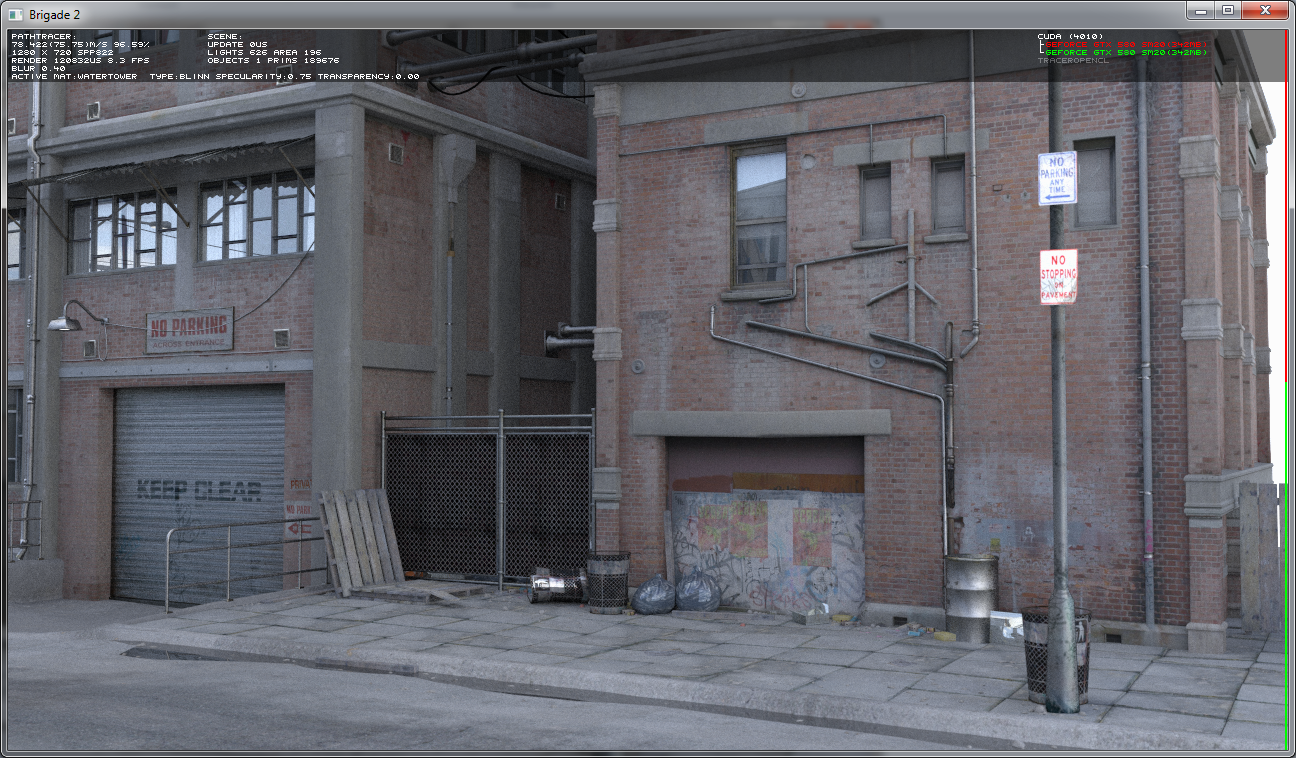
\includegraphics[scale = 0.15]{../figures/hd1.png}
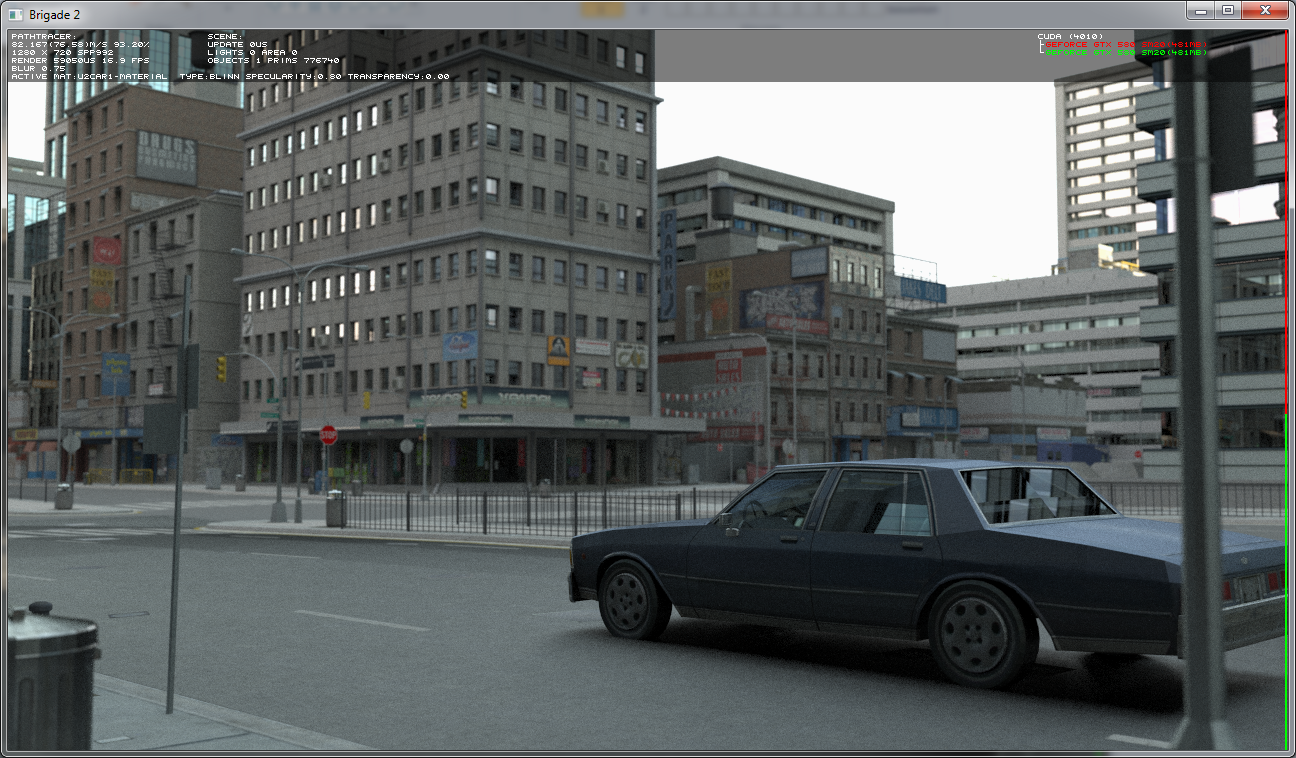
\includegraphics[scale = 0.15]{../figures/blinn5ed.png}

(Imágenes: Brigade 2 Renderer)


\end{frame}




\begin{frame}{Síntesis de la Imagen de una Escena}
Cada punto (o píxel) en una imagen de una escena a \textbf{renderizar}, debe computar la \textbf{radiancia} (o energía radiada) que arriba a la \textbf{cámara} desde toda la escena.

Cada objeto de la escena puede emitir radiancia, en todo el espectro electromagnético, hacia el observador.

La radiancia \textit{entrante} depende de numerosos factores, entre ellos la \textbf{forma} del objeto, el \textbf{material} del objeto, la \textbf{oclusión} existente entre el objeto y la cámara, su temperatura, etc.
\end{frame}



\begin{frame}[Luz]
\begin{block}{Luz}
\begin{itemize}
\item La comprensión del fenómeno evolucionó considerablemente a lo largo del tiempo.
\item Actualmente, se acuña el término ``dualidad onda-partícula'' para describirlo. El mismo es en extremo complejo, por lo tanto debe simplificarse su tratamiento en computación gráfica.
\item La primera simplificación se da teniendo en cuenta que, en la mayoría de los casos, sólo la \textbf{luz visible} es la que debe modelarse, ya que la misma define la apariencia del objeto.
\item La distribución de la luz visible en una escena se asume por medio de líneas rectas o \textbf{rayos}, es decir, se opta por la representación óptico geométrica del fenómeno, ya que se representará al mismo a escala macroscópica.
\end{itemize}
\end{block}
\end{frame}

\begin{frame}{}

\centering
%\includegraphics[scale = 0.15]{realidadVirtual.jpg}

\begin{block}{Sin embargo, este es sólo un paso de muchos}
\begin{itemize}
\item Debe modelarse, además, la interacción de la luz con \textbf{cada objeto} en particular.
\item Este problema es aún mayor ya que cada material se comporta de manera diferente.
\item El problema es doble: debe simularse la interacción de la luz con el material \textbf{Y} la geometría del mismo.
\end{itemize}
\end{block}

\end{frame}

\begin{frame}{Materiales}
?`Qué es la apariencia de un material?
\begin{itemize}
\item Definición informal: {\em percepción} del mismo por parte de una persona.
\item Conjunto de estímulos visuales.

%\item Se codifica en datos, estructuras de datos y algoritmos.
\end{itemize}

\centerline{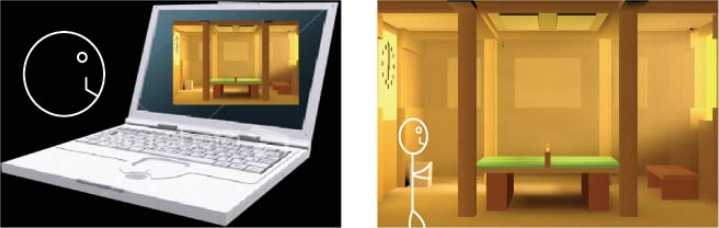
\includegraphics[scale = 0.25]{../figures/fotorealismo}}

El \textbf{foto-realismo} busca sintetizar imágenes que produzcan el \textbf{mismo efecto}, en la percepción, que aquél producido por la visualización de una fotografía del material/escena.
\end{frame}


\begin{frame}{Modelado de la Apariencia de Materiales}
\begin{block}{}
\begin{itemize}
\item El modelado de cada material depende de la escala buscada.
\item Microscópico: detalles que no son visibles al ojo humano. Se utilizan diversas técnicas estadísticas.
\item Macroscópico: detalles visibles al ojo humano. Se utilizan triángulos, texturas, etc.
\end{itemize}
\end{block}
El material debe ser estudiado para comprender su apariencia, a partir de la cual derivar un modelo numérico del mismo

\centerline{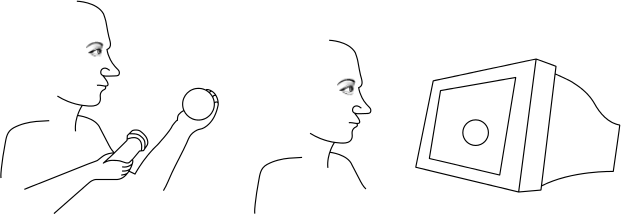
\includegraphics[scale = 0.25]{../figures/apariencia}}
\end{frame}

\begin{frame}
\begin{block}{}
Debido a las consideraciones anteriores, en esta tesis haremos hincapié en materiales \textbf{porosos}.

\begin{itemize}
\item Producir una geometría configurable, intuitiva y creíble de estos materiales.
\item Implementación de un modelo inspirado en procesos físicos en la formación de un material poroso: el pan.
\item Se busca renderización foto-realista en tiempo real.
\item Se busca validar los resultados.
\end{itemize}

La tesis presenta algunos resultados favorables inesperados
\begin{itemize}
\item Caracterización y clasificación de imágenes de pan
\item Generación de imágenes de materiales no porosos (madera, mármol..)
\end{itemize}


\end{block}
\end{frame}




\section{Trabajo Previo}

\begin{frame}
\begin{block}{}
\begin{center}
\vspace{1cm}
\huge{Trabajo Previo}
\vspace{1cm}
\end{center}
\end{block}
\end{frame}

\subsection{Materiales}

\begin{frame}{Materiales con mayor aparición en escenas}

En computación gráfica, los materiales para los cuales se ha desarrollado mayormente la literatura científica incluye al agua, la piel humana, metales y plásticos, entre otros. Esto se debe a la \textbf{facilidad del diseño}, a la necesidad de cierto \textbf{grado de realismo}, y a su \textbf{aparición constante en escenas}.

\end{frame}

\begin{frame}{Materiales con menor aparición en escenas}

Otros materiales, como es el caso de materiales cocidos, materiales porosos y materiales comestibles, presentan mayor complejidad en el modelado:

\begin{itemize}
\item \textbf{Geometría compleja y visible}, rica interacción con la luz: translucencia, reflexión, absorción, etc.
\item El ser humano puede \textbf{distinguir con facilidad} un modelo si el mismo no es tratado cuidadosamente.
\item El \textbf{costo computacional} de modelar y renderizar estos materiales resultaba excesivo hasta la aparición masiva del hardware paralelo.
\end{itemize}

Alan Fournier: `computer graphics has still not been
able to convincingly render a slice of bread' (2001). 


\end{frame}

\subsection{Modelado de la Geometría: Técnicas Procedimentales}
\begin{frame}{Modelado de la Geometría: Técnicas Procedimentales}

En determinados casos, el modelado por medio de supervisión humana repetitiva no es deseable.

\vspace{0.5cm}
Por ejemplo, al diseñar un bosque. Diseñar separadamente cada árbol requeriría un tiempo excesivo.

\vspace{0.5cm}
Debido a esto se desarrollaron técnicas artísticas, basadas en algoritmos, los cuales permiten diseñar geometrías de manera semi-automática, recibiendo el nombre de \textbf{Procedimentales}.

\end{frame}

\begin{frame}{Sistemas-L}
El botánico Lindenmayer estudió y acuñó estos sistemas para describir la estructura visible de plantas. Fue capaz de representar objetos complejos de manera convincente, utilizando un procedimiento muy sencillo de generación.

La estructura de una planta está representada por medio de una \textbf{cadena de caracteres}.
A través de un procedimiento recursivo de reemplazo de caracteres basados en reglas sencillas, se pueden generar estructuras complejas.

\end{frame}

\begin{frame}

La generación cuenta con un \textbf{axioma} y una o varias reglas \textbf{reglas de producción}.

Además, se especifica un número de iteraciones, donde en cada iteración se aplican reglas de producción a la cadena de caracteres resultante anterior.

\vspace{1cm}

Ejemplo:

Axioma: $F$

$P1: F \rightarrow FfF$

Produce las derivaciones:
$F \rightarrow FfF \rightarrow \textbf{FfF}f\textbf{FfF} \ldots$

\end{frame}

\begin{frame}{Sistemas-L: Ejemplo y ``Renderización''}
Dado un estado inicial ($x$,$y$,$90^{\circ}$), el \textbf{axioma} F, y una regla de producción $F \rightarrow FF-FfF-FF$, donde

\begin{itemize}
\item F, moverse hacia adelante un paso $d$, dibujando,
\item f, moverse hacia adelante un paso $d$, sin dibujar,
\item +, rotar un ángulo $\delta$,
\item -, rotar un ángulo $-\delta$.
\end{itemize}

\center
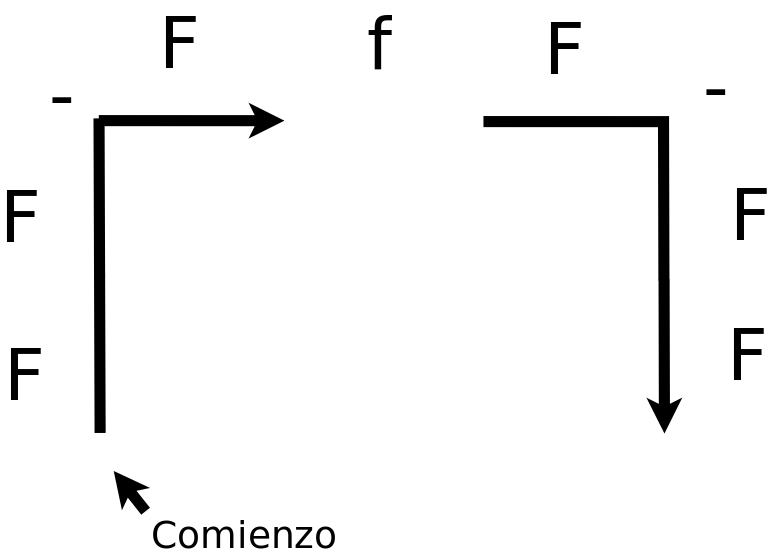
\includegraphics[width=5cm]{../figures/tortuga}

\end{frame}

\begin{frame}{Sistemas-L: Arboles}
Por medio de una pila de estados, donde el caracter $[$ se utiliza para copiar el estado actual en la pila (operación {\em push}), y el caracter $]$ implica un reemplazo del estado actual por el de la cabeza de la pila ({\em pop}):


\center
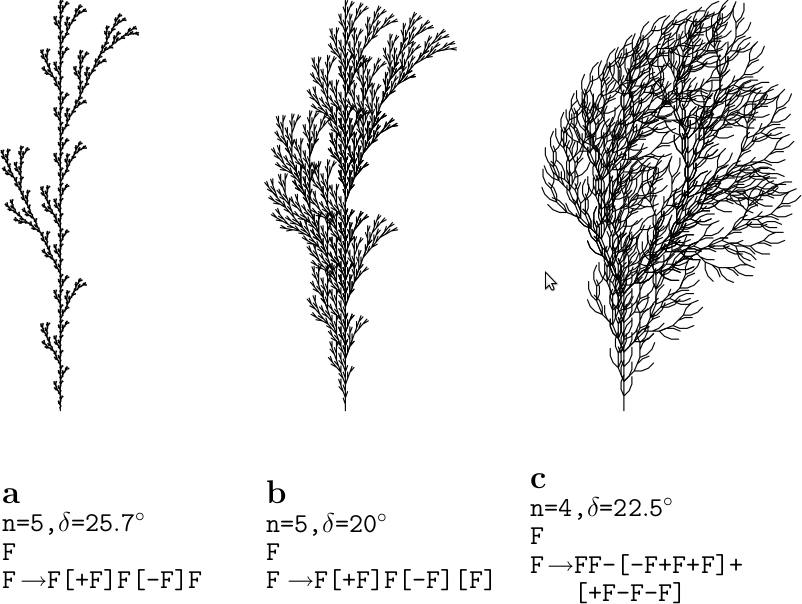
\includegraphics[width=6.3cm]{../figures/sistemalcorchete}

\end{frame}

\begin{frame}{Sistemas-L: Arboles 3D}
\center
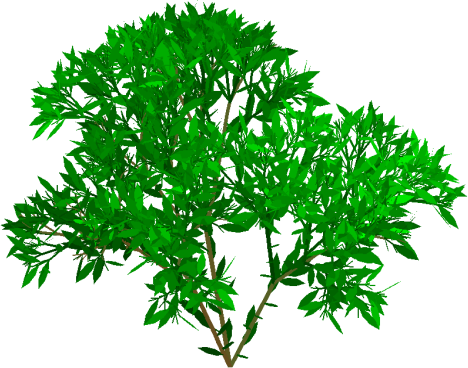
\includegraphics[width=6.3cm]{../figures/3dlsystem}

\end{frame}

\begin{frame}
Este ejemplo se basa en un modelado basado en la \textbf{similaridad} entre el objeto sintético resultante y el objeto real.

\vspace{1cm}

Sin embargo, es posible obtener representaciones más precisas atendiendo a procesos de formación de materiales.
\end{frame}

\subsection{Modelado Físico de materiales}

\begin{frame}{Modelado Físico de materiales}

Por medio de ecuaciones del \textbf{comportamiento} o \textbf{crecimiento} de los mismos, es posible obtener aproximaciones computacionales \textbf{más precisas}.

Las \textbf{ecuaciones de Navier-Stokes} se utilizan en la simulación realista de fluídos

Dadas condiciones iniciales para $\bold{u}$ y $p$ cuando $t = 0$, la evolución de las cantidades puede describirse como sigue, independientemente del número de dimensiones,

\begin{align*}
\nabla \cdot \bold{u} &= 0\\
\frac{\partial \bold{u} }{\partial t} &= - (\bold{u} \cdot \nabla) \bold{u} - \frac{1}{\rho} \nabla p + \nu \nabla^{2} \bold{u} + \bold{f},
\end{align*}

\noindent donde $\nu$ representa la viscosidad cinemática del fluido, $\rho$ la densidad y $\bold{f}$ una fuerza externa.

\end{frame}

\begin{frame}{Ecuaciones de Navier-Stokes, humo}
\center
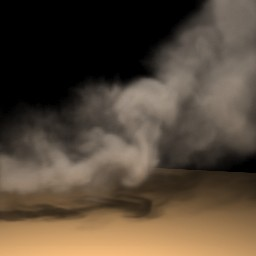
\includegraphics[width=6.3cm]{../figures/smoke}

\end{frame}

\begin{frame}

Hasta aquí dimos ejemplos del modelado de la \textbf{geometría} de los materiales.

\vspace{0.5cm}
La geometría debe \textbf{renderizarse} para ser visualizada.
\vspace{0.5cm}

A continuación presentamos las ecuaciones necesarias para lograr representar el comportamiento de la luz en una escena, y por lo tanto, necesarias para obtener imágenes realistas de la interacción de estas geometrías con la luz.

\end{frame}

\subsection{Renderizado}

\begin{frame}
De acuerdo al tipo de material a renderizar, existen dos clases principales de técnicas de modelado:

\begin{block}{}
\begin{itemize}
\item Superficies (Metales, plásticos)
\item Volúmenes (Humo, fuego)
\end{itemize}
\end{block}
\end{frame}


\begin{frame}{Ecuación del Renderizado de Superficies}
La misma modela la \textbf{radiancia} entrante en un punto $x$ a través de \textbf{todas} las superficies $s_{i}$ de la escena, pasando por \textbf{todos} los puntos $x'$ de todas las superficies.
\begin{equation*}
L(\bold{x'} \rightarrow \bold{x}) =  g(\bold{x'}  \rightarrow \bold{x})  \left[ \epsilon(\bold{x'}  \rightarrow \bold{x}) + \int_{s}{\rho(\bold{x''}  \rightarrow \bold{x'}  \rightarrow \bold{x})L(\bold{x''}  \rightarrow \bold{x}) d\bold{x''}} \right]
\end{equation*}
donde $L(\bold{x'} \rightarrow \bold{x})$ representa la intensidad de la luz que viaja del punto tridimensional $\bold{x'}$ al punto $\bold{x}$ (sin oclusiones), $g(\bold{x'} \rightarrow \bold{x})$ un termino geométrico que modela la oclusión que podría existir entre $\bold{x}$ y $\bold{x'}$, $\epsilon(\bold{x'} \rightarrow \bold{x})$ la intensidad de la luz emitida desde $\bold{x'}$ a $\bold{x}$, $\rho(\bold{x''}  \rightarrow \bold{x'}  \rightarrow \bold{x})$ la intensidad de la luz emitida de $\bold{x''}$ a $\bold{x}$ por medio de una superficie en $\bold{x'}$ (esta cantidad será llamada función bidireccional de distribución de reflectancia, BRDF), y $S=\bigcup{s_{i}}$ la unión de todas las superficies $s_{i}$ de la escena
\end{frame}

\begin{frame}{Ecuación del Renderizado de Superficies}
\begin{wrapfigure}{l}{6cm}
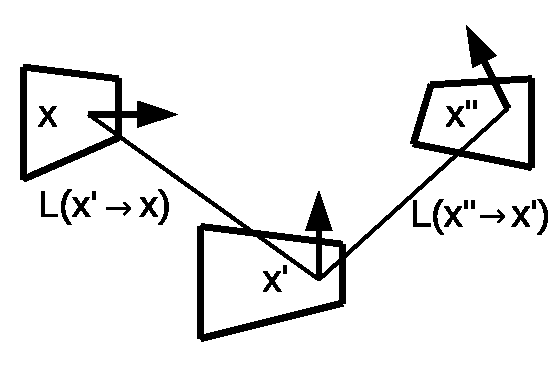
\includegraphics[scale = 0.6]{../figures/rendequation}
\end{wrapfigure}

Es recursiva, ya que la \textbf{energía radiante saliente} de un punto $x'$ depende de la \textbf{energía radiante entrante} desde todos los puntos de todas las superficies a ese punto.
De esta forma, $\bold{x}$,$\bold{x'}$ y $\bold{x''}$ varían sobre todas las superficies de la escena.
%Además se asume una superficie $S_{0}$, la cual se modela como una semi-esfera que engloba a toda la escena.

La ecuación aproxima las propiedades óptico-geométricas de las ecuaciones del electromagnetismo de Maxwell.

(Ray Tracing, Path Tracing)
\end{frame}


\begin{frame}{Ecuación del Renderizado de Volúmenes}
La misma expresa que el cambio ($\nabla$) de radiancia $L$ de un rayo de luz en un medio, en una dirección dada ($\vec{\omega}$) está dado por cuatro fenómenos: absorción, dispersión saliente, emisión (del medio) y dispersión entrante.
\begin{equation*}
\begin{aligned}
(\vec{\omega} \cdot \nabla) L(\bold{x} \rightarrow \vec{\omega}) = - \sigma_{a}(\bold{x}) L(\bold{x} \rightarrow \vec{\omega}) - \sigma_{s}(\bold{x}) L(\bold{x} \rightarrow \vec{\omega}) + \\
\sigma_{a}(\bold{x}) L_{e}(\bold{x} \rightarrow \vec{\omega}) + \sigma_{s}(\bold{x}) L_{i}(\bold{x} \rightarrow \vec{\omega}).
\end{aligned}
\end{equation*}
donde $\sigma_{a}$: coeficiente de absorción del medio, $\sigma_{s}$: coeficiente de dispersión del medio.

\end{frame}

\begin{frame}{Ecuación del Renderizado de Volúmenes}
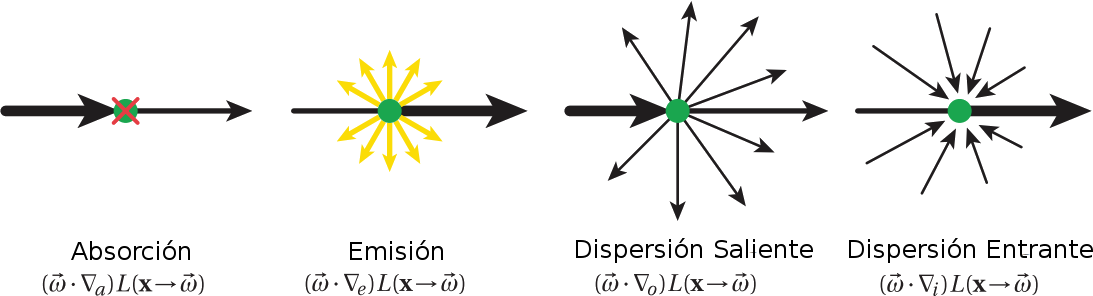
\includegraphics[scale = 0.55]{../figures/fenomenosrte}

Ray Casting (Direct Volume Rendering)
\end{frame}



\subsection{Materiales porosos}


\begin{frame}{Materiales porosos - Trabajo Previo}
La literatura utiliza ambos enfoques para producir materiales porosos. Cada uno de ellos con ventajas y desventajas.

\ \\

Volúmenes
\begin{block}{}
\begin{itemize}
\item permiten \textbf{cortes arbitrarios} en el objeto
\item son generalmente \textbf{más costosos}, tanto en almacenamiento como en tiempo de renderizado.
\end{itemize}
\end{block}
\end{frame}

\begin{frame}{Materiales porosos - Trabajo Previo}
Los modelos actuales de generación de geometría de materiales porosos en el área resultan de procesos artísticos.
Se utilizan diversos ruidos, como los ruidos de Voronoi, Perlin y Worley. Sin embargo, los métodos deben combinarse con otras consideraciones ad-hoc.

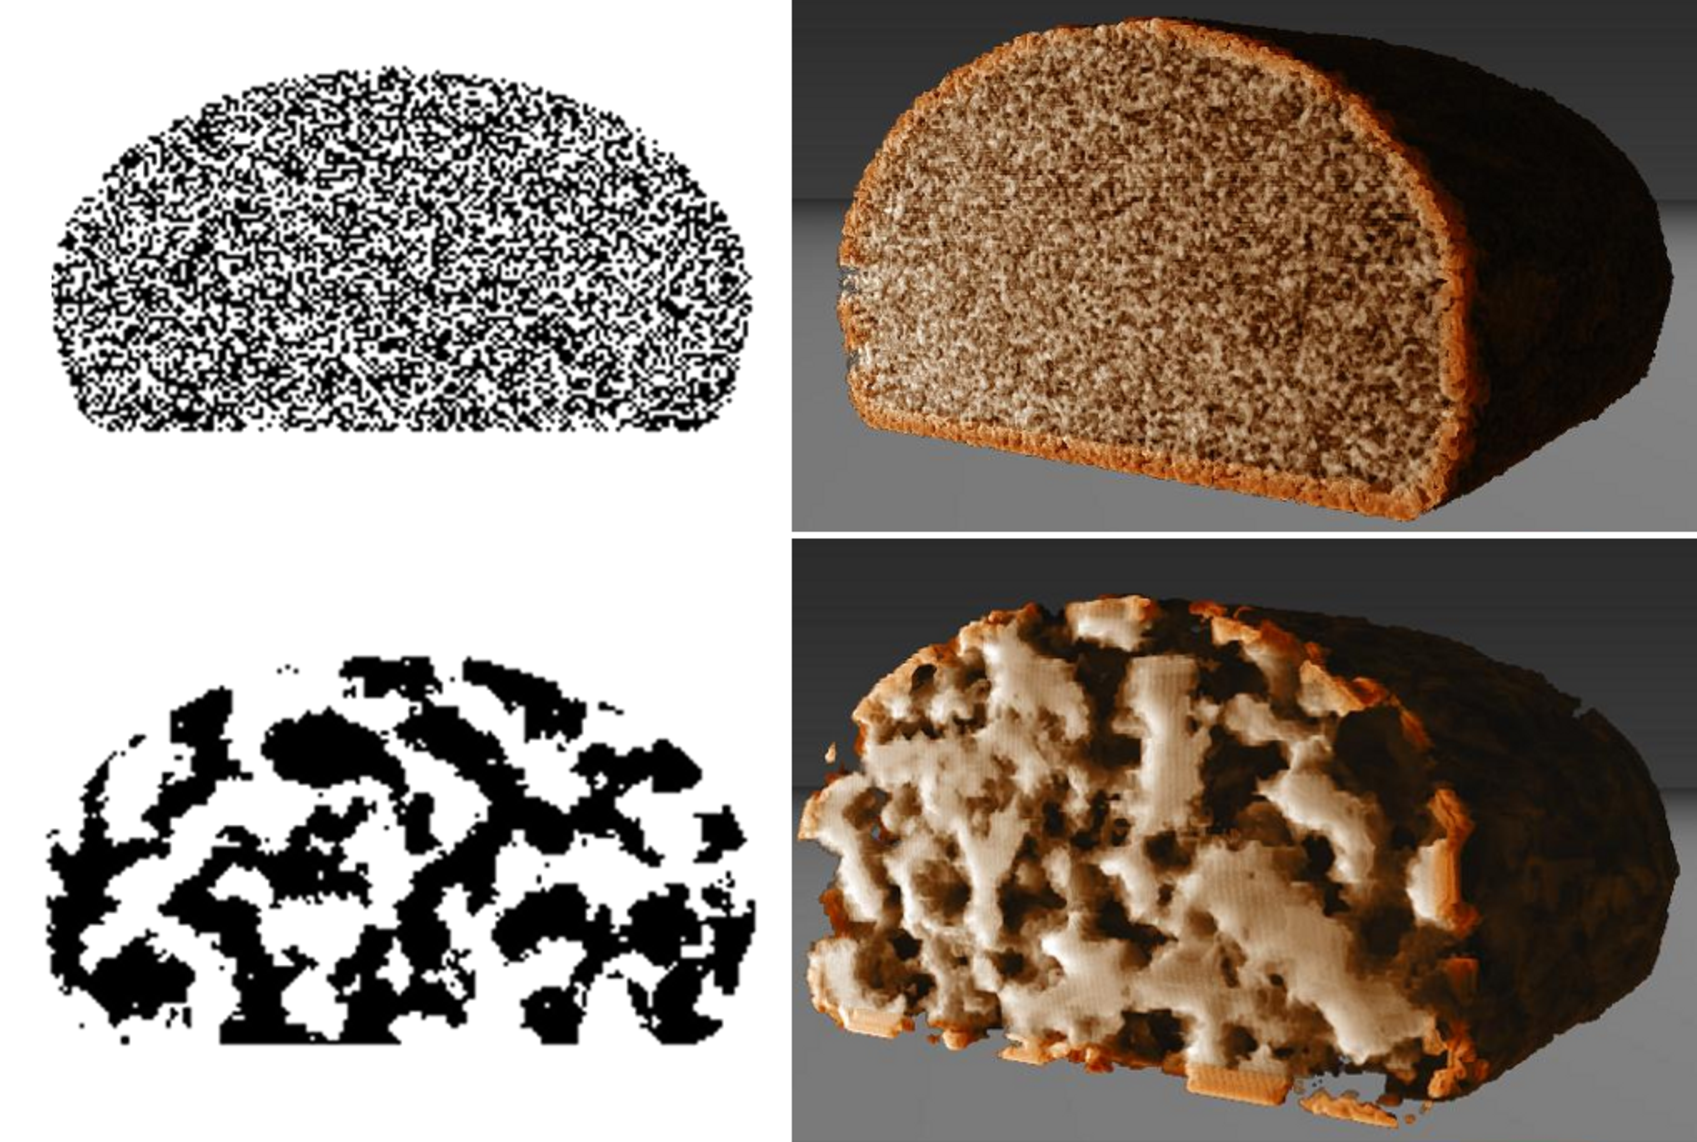
\includegraphics[scale = 0.2]{../figures/Fig8}
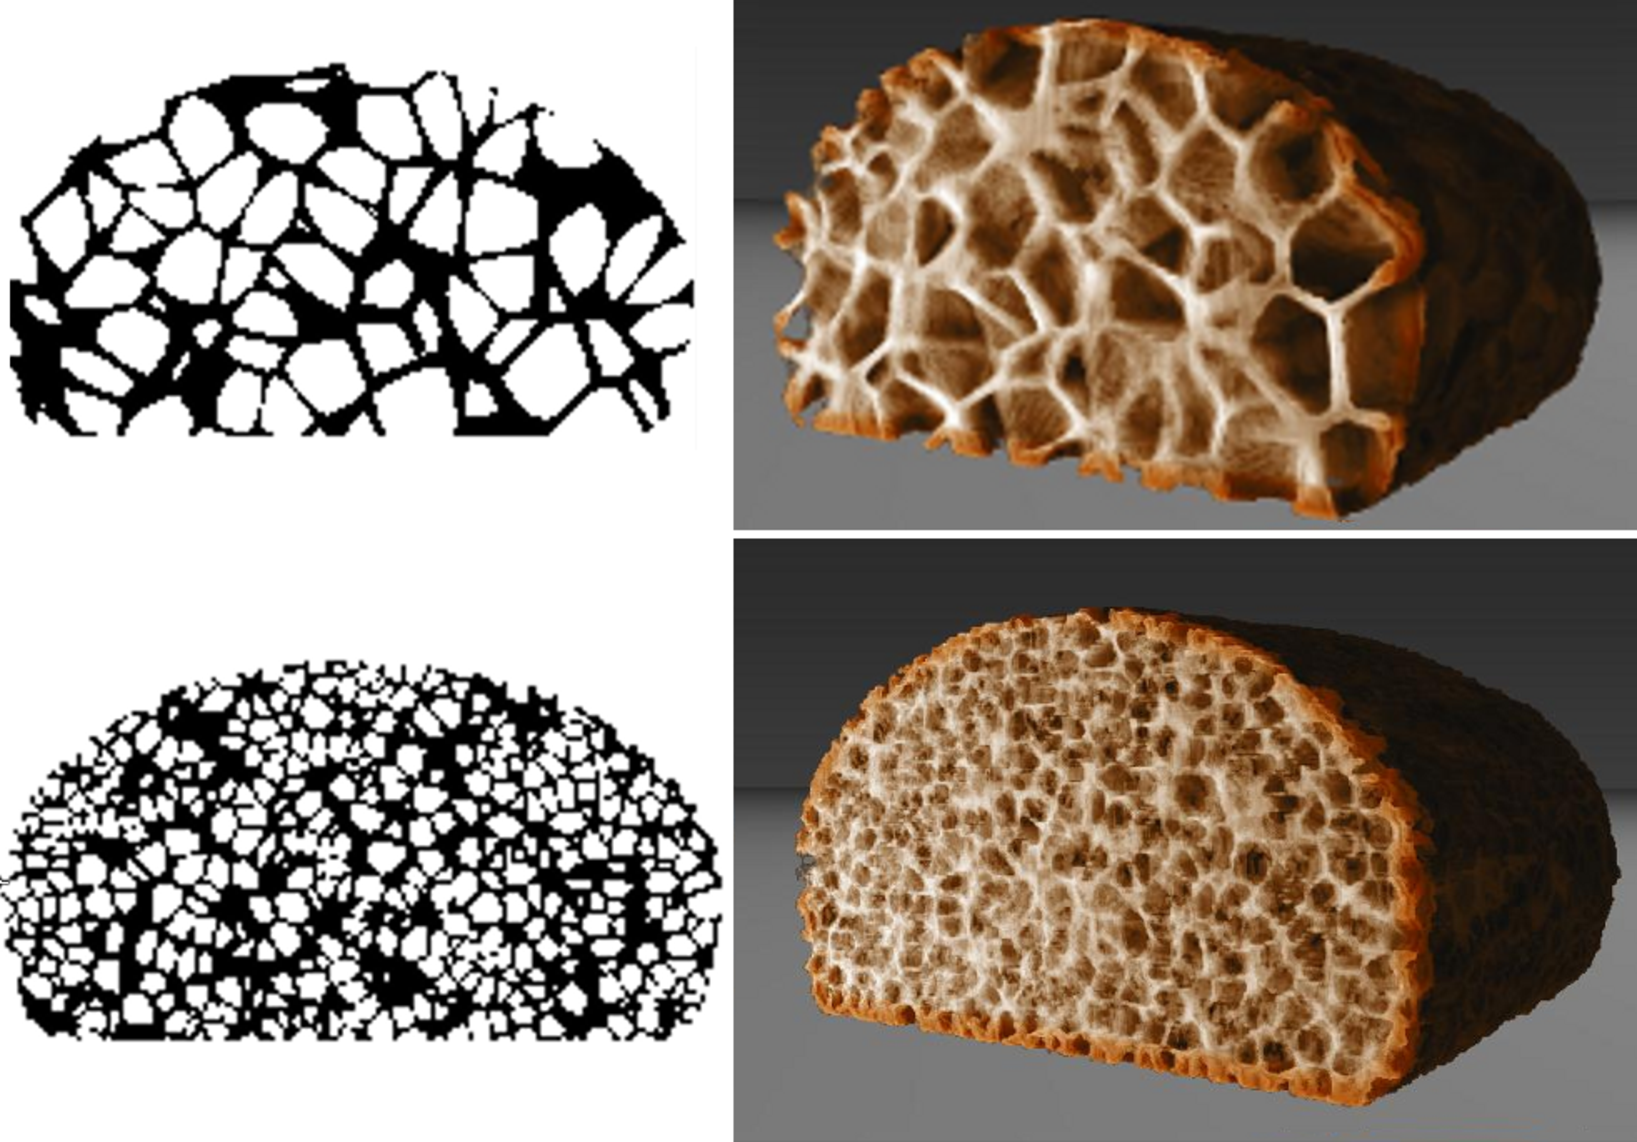
\includegraphics[scale = 0.2]{../figures/Fig9CAVW}

Ratatouille (Película): modelo de pan basado en ruido de Voronoi + un mapa indicando deformación de burbujas.
\end{frame}


\begin{frame}{Materiales porosos - Trabajo Previo}
Desventajas: 
\begin{block}{}
\begin{itemize}
\item control sobre cantidad y tamaño de las burbujas
\item deformación de burbujas
\item el usuario debe ser experto
\end{itemize}
\end{block}

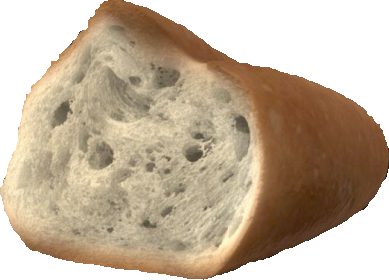
\includegraphics[scale = 0.3]{../figures/ratatouille}

\end{frame}

\begin{frame}

Modelo fenomenológico: Tong et al (2005), "Modeling and Rendering of quasi-homogeneous Materials"

Capturas sobre materiales reales utilizando cámaras y lásers $\rightarrow$ se obtienen distribuciones precisas de radiancia en el material.

\begin{itemize}
\item Proceso de captura muy complejo
\item Limitado a una geometría
\item Tiempos de cómputo no claramente establecidos
\item Imposibilidad de realizar cortes
\end{itemize}

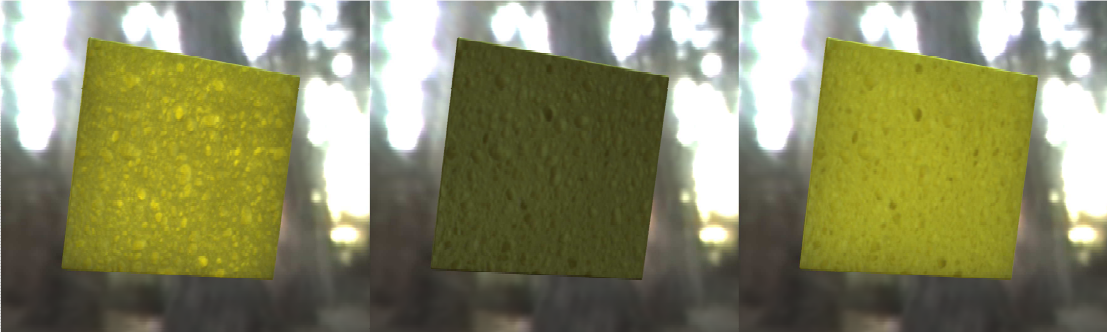
\includegraphics[scale = 0.3]{../figures/esponja}

\end{frame}


\section[Mod. de Materiales Porosos]{Modelado Procedimental de Materiales Porosos}

\begin{frame}
\begin{block}{}
\begin{center}
\vspace{1cm}
\huge{Modelado Procedimental de Materiales Porosos}
\vspace{1cm}
\end{center}
\end{block}
\end{frame}

\subsection{Modelado Procedimental de Materiales Porosos}
\begin{frame}{Modelado de Geometrías Porosas - Propuesta}
Presentamos un modelo de generación de geometrías porosas basados en:
\begin{itemize}
\item Sistemas de Partículas que crecen, evitándose
\item Sistemas dinámicos como medio de crecimiento
\end{itemize}
\end{frame}

\begin{frame}{Sistemas de partículas}
Características
\begin{itemize}
\item Conjunto de \textbf{partículas}: una partícula posee posición, dirección, color, tiempo de vida, etc.
\item Utilizado para representar fluídos, y objetos con interfaces sin definición precisa

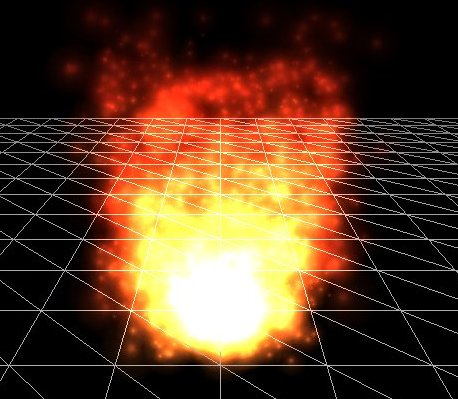
\includegraphics[scale = 0.3]{../figures/fire}
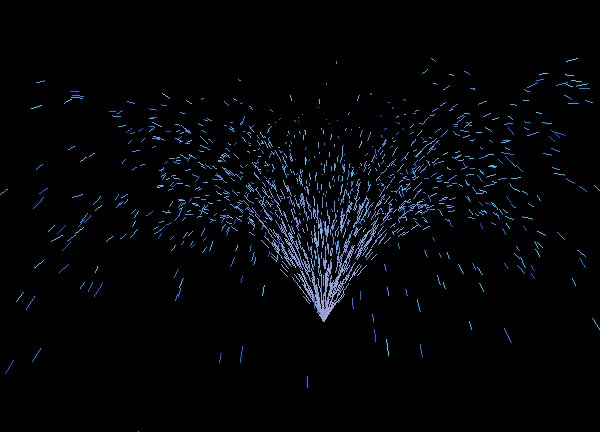
\includegraphics[scale = 0.277]{../figures/fireworks}
\end{itemize}
\end{frame}

\begin{frame}
El sistema consta de un conjunto de partículas $P$, y dos grillas, $L$, y $L^{2}$:
\begin{align*}
  P = \{p_{1}, ... , p_{n}\}, n  \in \mathbb{N}, \\
  L_{N\times N \times N},\\
  L^{2}_{N\times N \times N},\\ N \in \mathbb{N}.
\end{align*}

inicialmente $L_{xyz}=1$: masa

inicialmente $L^{2}_{xyz}=-1$: celda libre,

Cada partícula posee:
\begin{equation*}
  p_{i} = \{O_{i}, C_{i}\}, 1 \le i \le n,
\end{equation*}

\begin{itemize}
\item $O_{i} = \{o_{1}, ... , o_{n_{i}}\}$:posiciones ocupadas por la part\'icula en $L$.

\item $C_{i} = \{c_{1}, ... , c_{m_{i}}\}$:posiciones en el {\em contorno} de la part\'icula en $L$.
\end{itemize}

\end{frame}

\begin{frame}

\begin{algorithm}[H]
\begin{algorithmic}[1]
        \IF {$vacio?~C[i]$}
            \STATE{morir()}
        \ENDIF
        \FOR{$h \in C[i]$}
            \STATE{$C[i].eliminar(h)$}
            %\COMMENT{la posición ya fue explorada}
            %\STATE{// Si la pos. o contorno pertenecen a otra partícula, descartar}
            %\STATE{// borde\_libre chequea disponibilidad en el vecindario}
            \IF{$!(L^{2}[h] > 0 ~\&\&~ L^{2}[h] != i) ~\&\&~ borde\_libre(h,separacion)$}
                %\State{// Posición libre, ocupar}                
                \STATE{$L[h] \gets 0$} %\COMMENT{masa -> aire}
                \STATE{$O[i].agregar(h)$}
                \STATE{$C[i].agregar(vecindario(h))$} 
                \STATE{$L^{2}.setear(vecindario(h),i)$} %\COMMENT{Marcar posiciones en $L^{2}$ como $i$}
                \STATE{$L^{2}.setear(h,i)$}
                \STATE{Break}
                %\Comment{turno de la partícula $i+1$...}
            \ENDIF
        \ENDFOR
\end{algorithmic}
%\label{alg:seq}
\end{algorithm}
\end{frame}

\begin{frame}
La partícula 14 marcó en su contorno celdas previamente marcadas por la partícula 7 en su contorno
\centerline{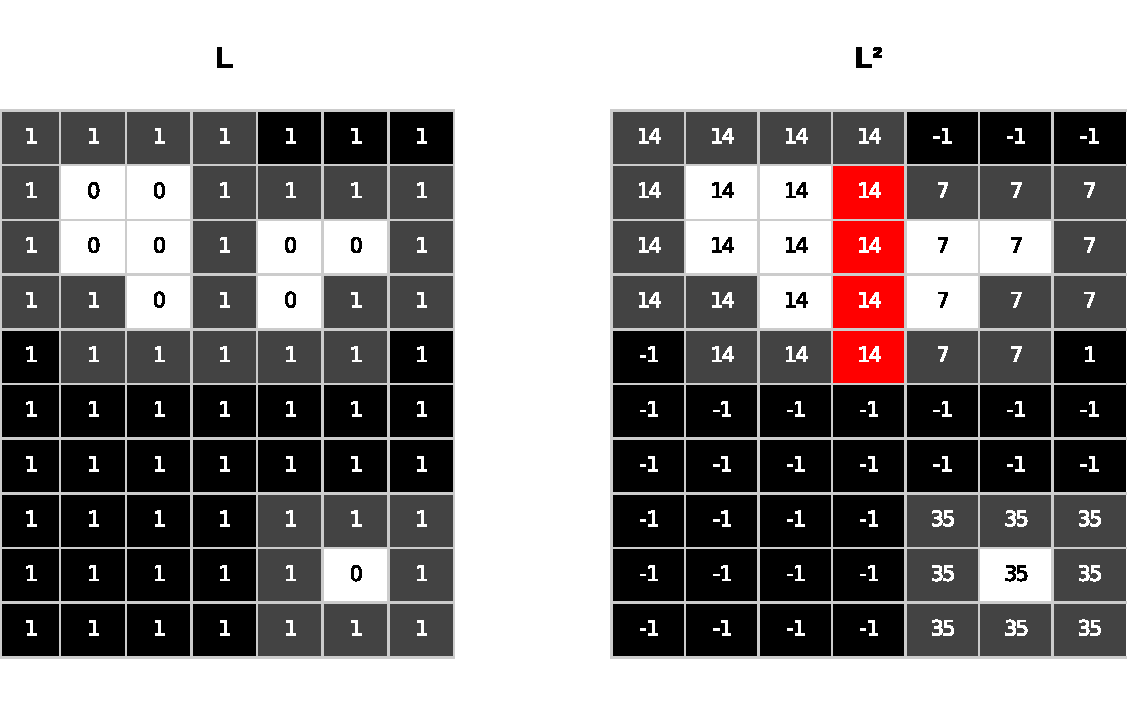
\includegraphics[scale = 0.45]{../figures/sistemaparticulas}}
La partícula 14 \textbf{no} tomará las posiciones en rojo, ya que \textbf{borde\_libre} chequea que su contorno no pertenezca a otra partícula
\end{frame}

\begin{frame}{Ejemplo: crecimiento}
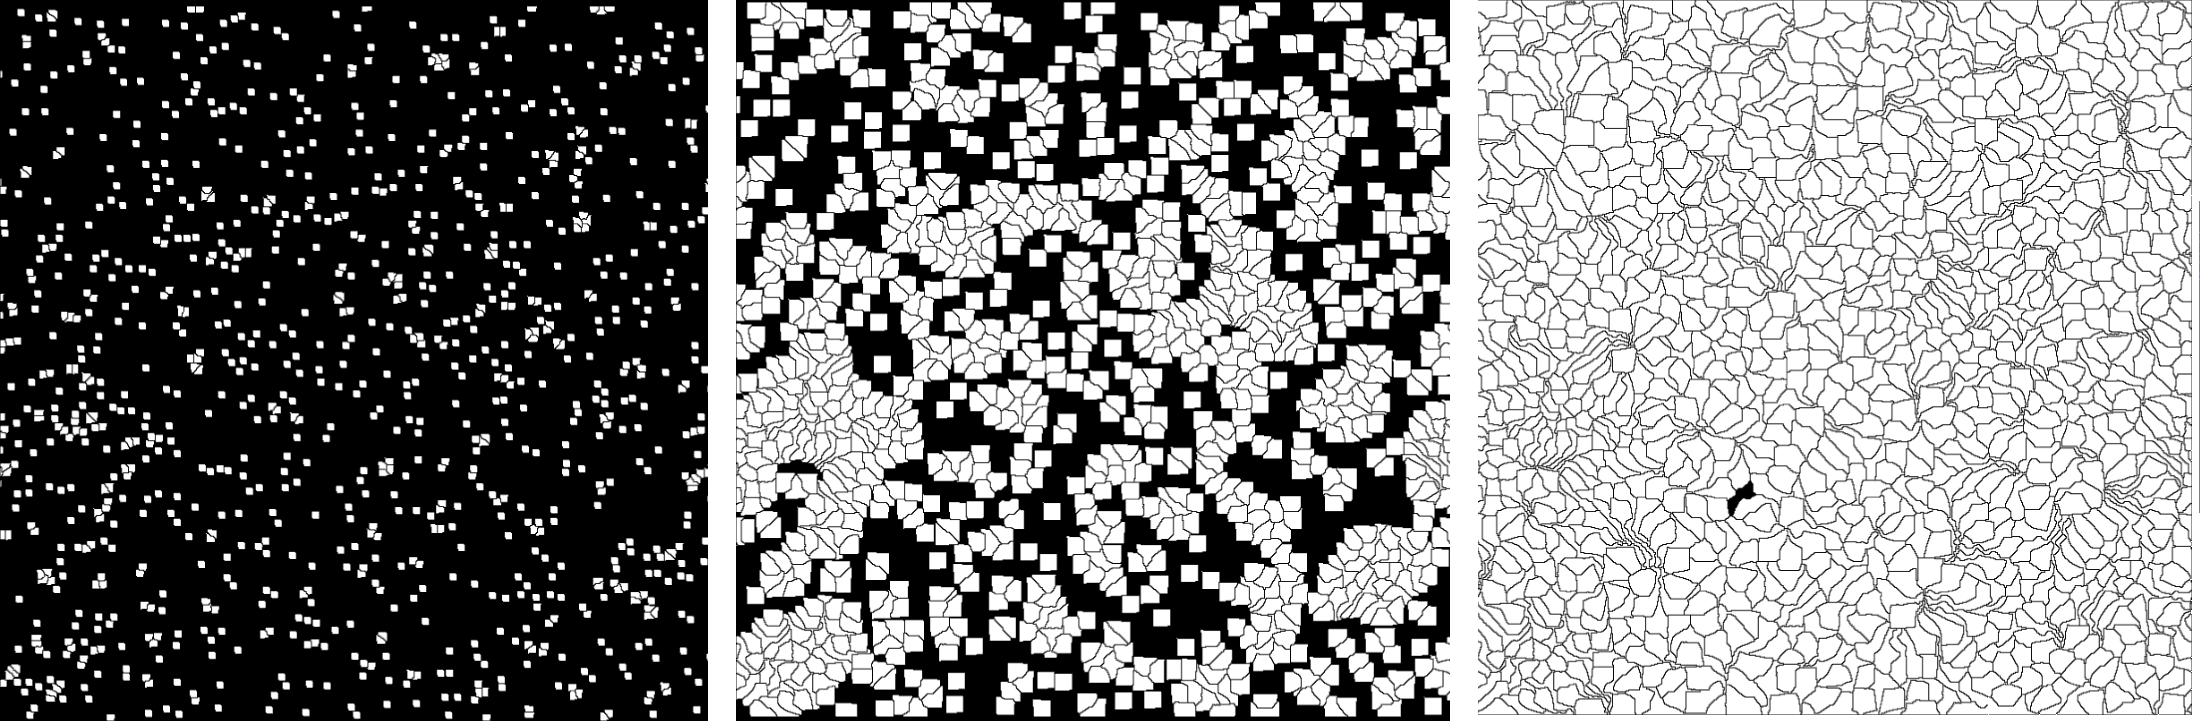
\includegraphics[scale = 0.15]{../figures/modeladocrec}
\end{frame}


\begin{frame}{Sistemas dinámicos}

De manera general, las ODEs se representan utilizando el siguiente sistema de ecuaciones:
\begin{equation*}
  \begin{aligned}
    \dot{x_{1}} = f_{1}(x_{1},\ldots,x_{n}),\\
    \ldots\\
    \dot{x_{n}} = f_{n}(x_{1},\ldots,x_{n}),
  \end{aligned}
\end{equation*}



\end{frame}


\begin{frame}{Crecimiento}
El crecimiento de las partículas puede ser aleatorio o direccionado.

Un campo vectorial (discreto), definido por un Sistema Dinámico (SD), puede utilizarse para direccionar las partículas 

Ejemplo de SD en dos dimensiones (imagen de la izquierda),
\begin{equation*} \label{eq:simple}  
  \begin{aligned}
    \dot{x} &= x^{2}-y^{2}+1,\\
    \dot{y} &= 2xy+1.
  \end{aligned}
\end{equation*}
  \centerline{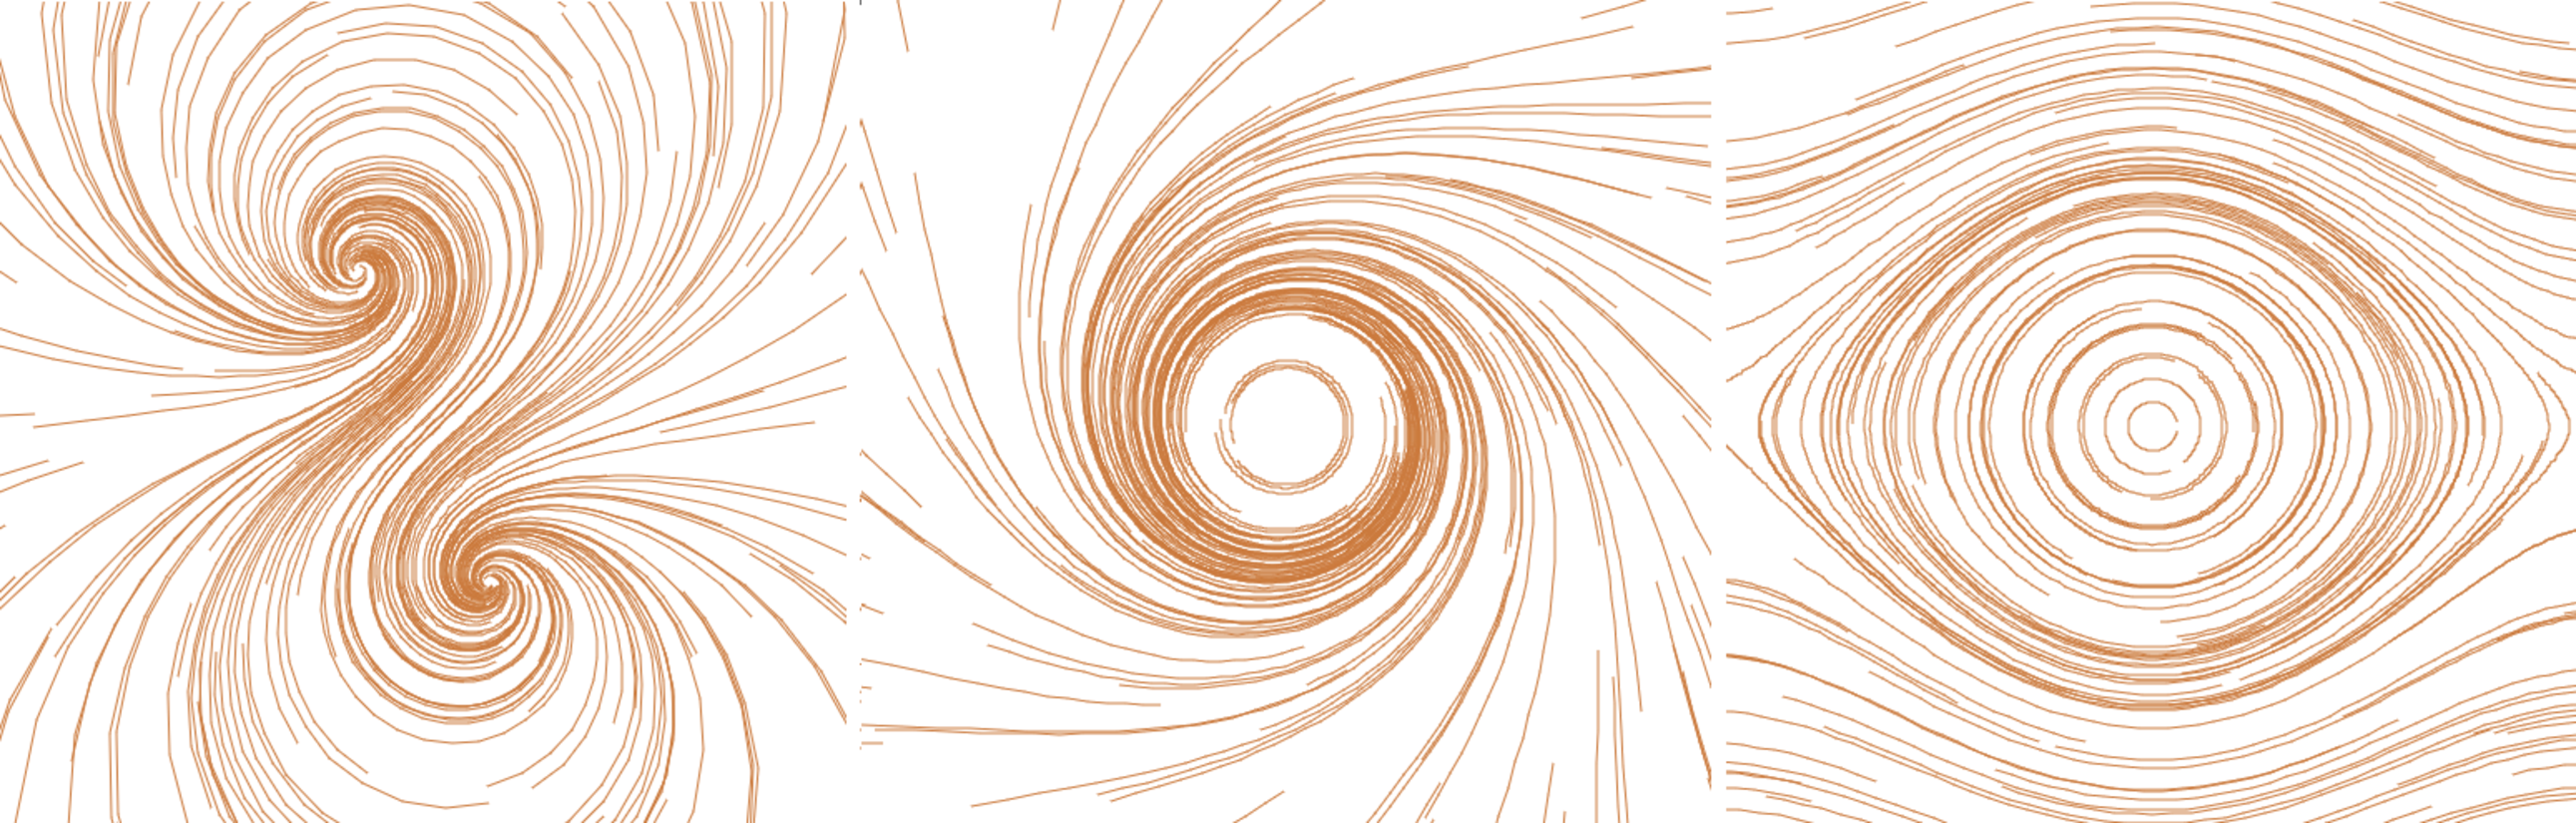
\includegraphics[width=9cm]{../figures/Fig2}}
\end{frame}

\begin{frame}
\begin{algorithm}[H]
\begin{algorithmic}[1]
\STATE $solucion = round(Runge\_Kutta(h))$
%\Comment {Se calcula la siguiente posición}
\STATE $vec = vecindario(h)$
\STATE $mejor = abs(vec[0] - solucion)$
\STATE $elegida = h$
\STATE $vec.eliminar(h)$
\FOR {$w \in vec$}
%\STATE{// Se calcula la posición del vecindario que mejor aproxima al sistema}
    \IF {$abs(vec[w]-solucion) < mejor$}
        \STATE $mejor = abs(vec[w]-solucion)$
        \STATE $elegida = w$
    \ENDIF
    \IF {$aleatorio() < aleatoriedad$} 
    %\Comment {$0 <= aleatorio() <= 1$}
        \STATE $C[i].agregar(w)$
    \ENDIF
\ENDFOR
%\State{// Se agrega al vecindario sólo la posición que mejor aproxima la solución}
\STATE $C[i].agregar(elegida)$
\end{algorithmic}
\end{algorithm}
\end{frame}

\begin{frame}{Sistemas de partículas + Sistemas Dinámicos}
Utilizando distintos parámetros de aleatoriedad en el crecimiento, se obtienen distintas apariencias.

En las imágenes, aleatoriedad = 0.3, 0.2, y 0.1
  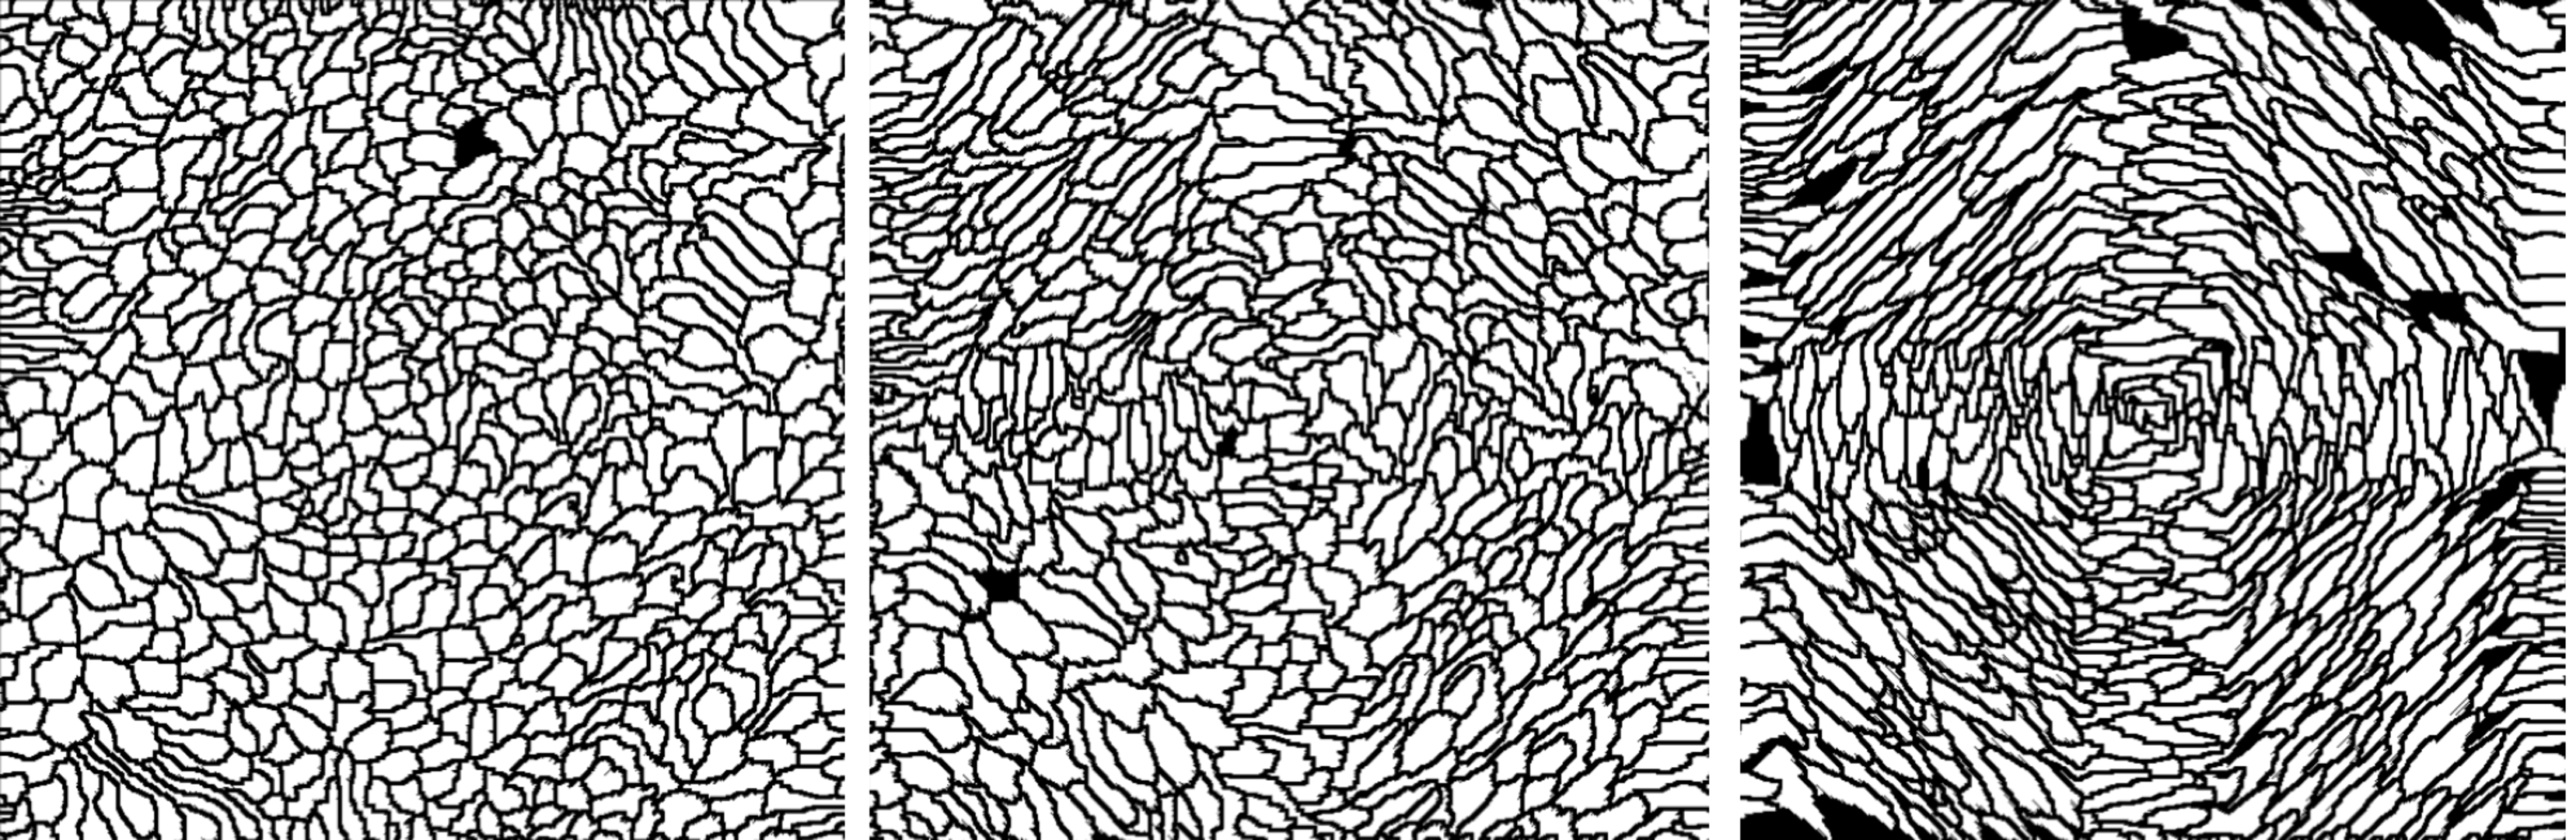
\includegraphics[width=12cm]{../figures/Fig3}
\end{frame}

\begin{frame}{Mapa de Distancias}

Dada una textura volumétrica $M$, el algoritmo genera una textura volumétrica a valores reales $DF_{M}$ con las mismas dimensiones que $M$,


$$DF_{M}[i,j,k] = \min \bigg\{ \delta([i,j,k],[i',j',k']): M[i',j',k'] = 0 \bigg\},$$


\noindent donde $[i,j,k]$ y $[i',j',k']$ son celdas en las respectivas texturas, representando las posiciones espaciales $(i,j,k)$ y $(i',j',k')$, y $\delta$ es la función que computa la distancia entre dos celdas, las cuales pueden ser la distancia de Manhattan, o la distancia Euclidiana.

\end{frame}

\begin{frame}{Mapa de Distancias}

\centerline{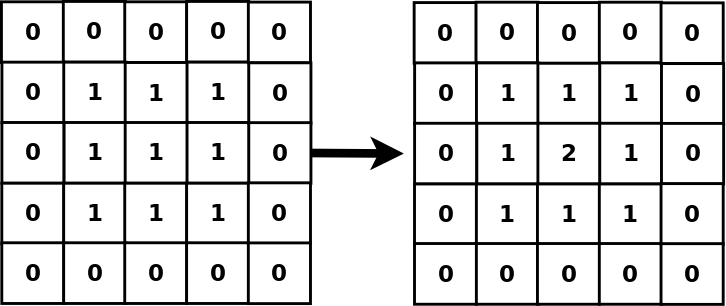
\includegraphics[width=12cm]{../figures/distance}}

\end{frame}

\begin{frame}{Condiciones de contorno}
Dada una geometría tridimensional \textbf{arbitraria}, se elige un eje Cartesiano ($x$, $y$ o $z$) y se computan cortes bidimensionales sobre ese eje.

Para cada corte se establecen condiciones de contorno, a través de un campo vectorial discreto que ``sigue'' al contorno

Ortogonal al gradiente del corte.

  \centerline{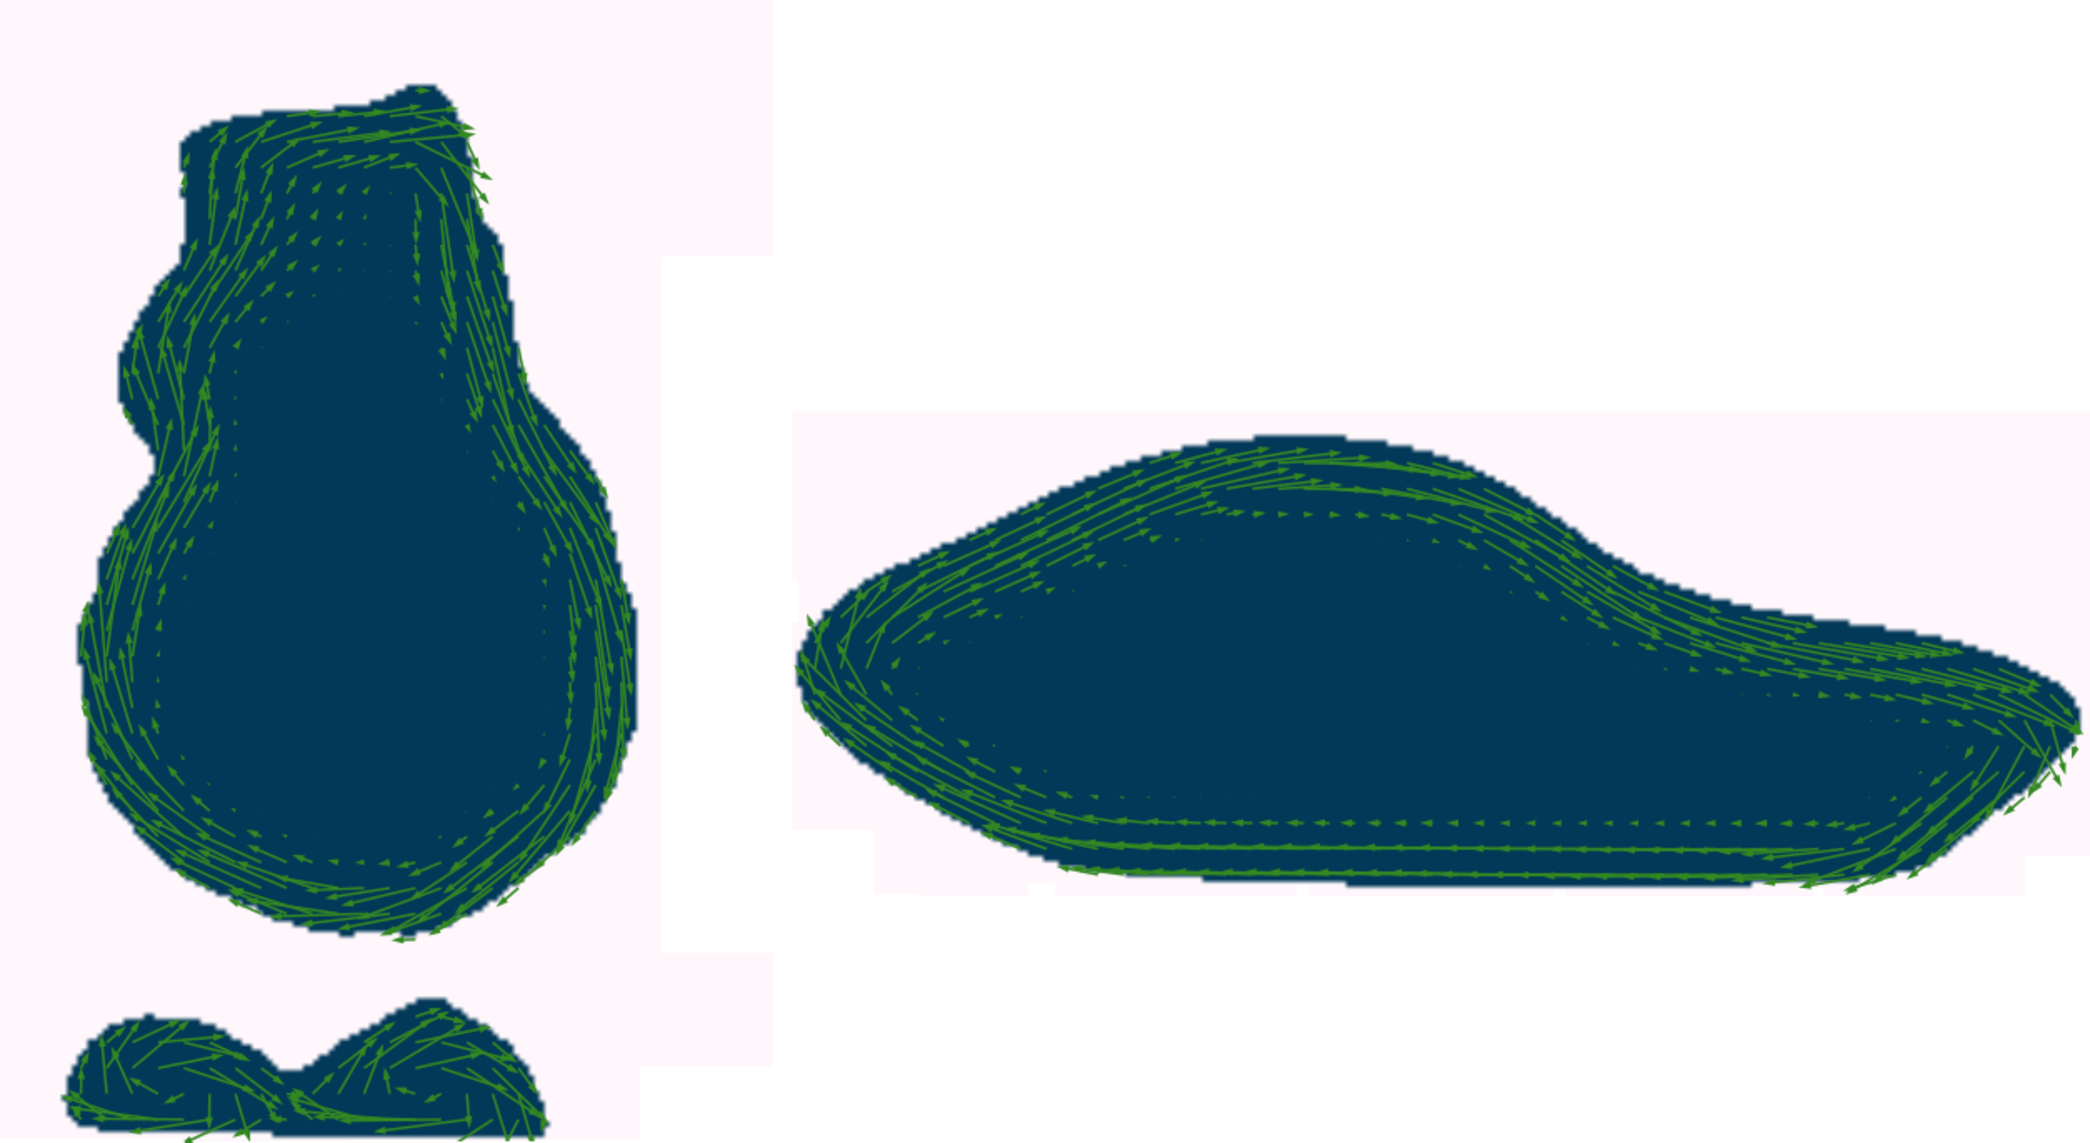
\includegraphics[width=8cm]{../figures/Fig4}}
\end{frame}

\subsection{Resultados}

\begin{frame}{Resultados}
Finalmente se centra el sistema dinámico en el {\em centro de masa} de cada corte, y junto a las condiciones de contorno, definen un patrón natural para el corte.

Si bien esta elección no representa una parametrización completamente tridimensional, resulta más intuitivo definir un sistema dinámico en dos dimensiones.

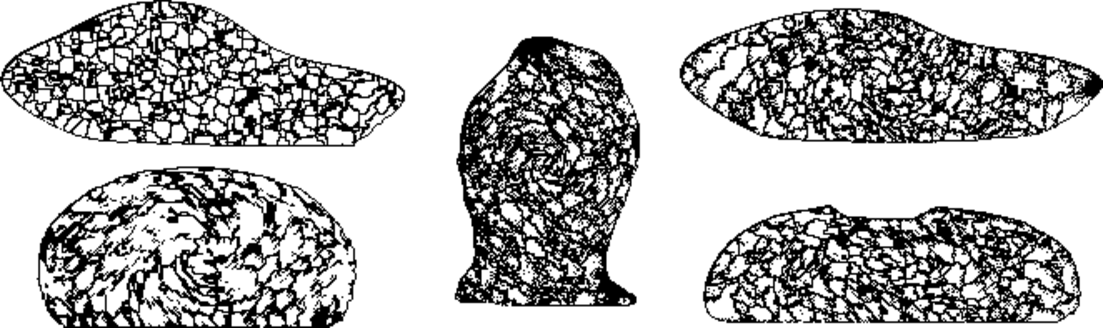
\includegraphics[width=12cm]{../figures/Fig5}
\end{frame}

\begin{frame}{Resultados}
\centerline{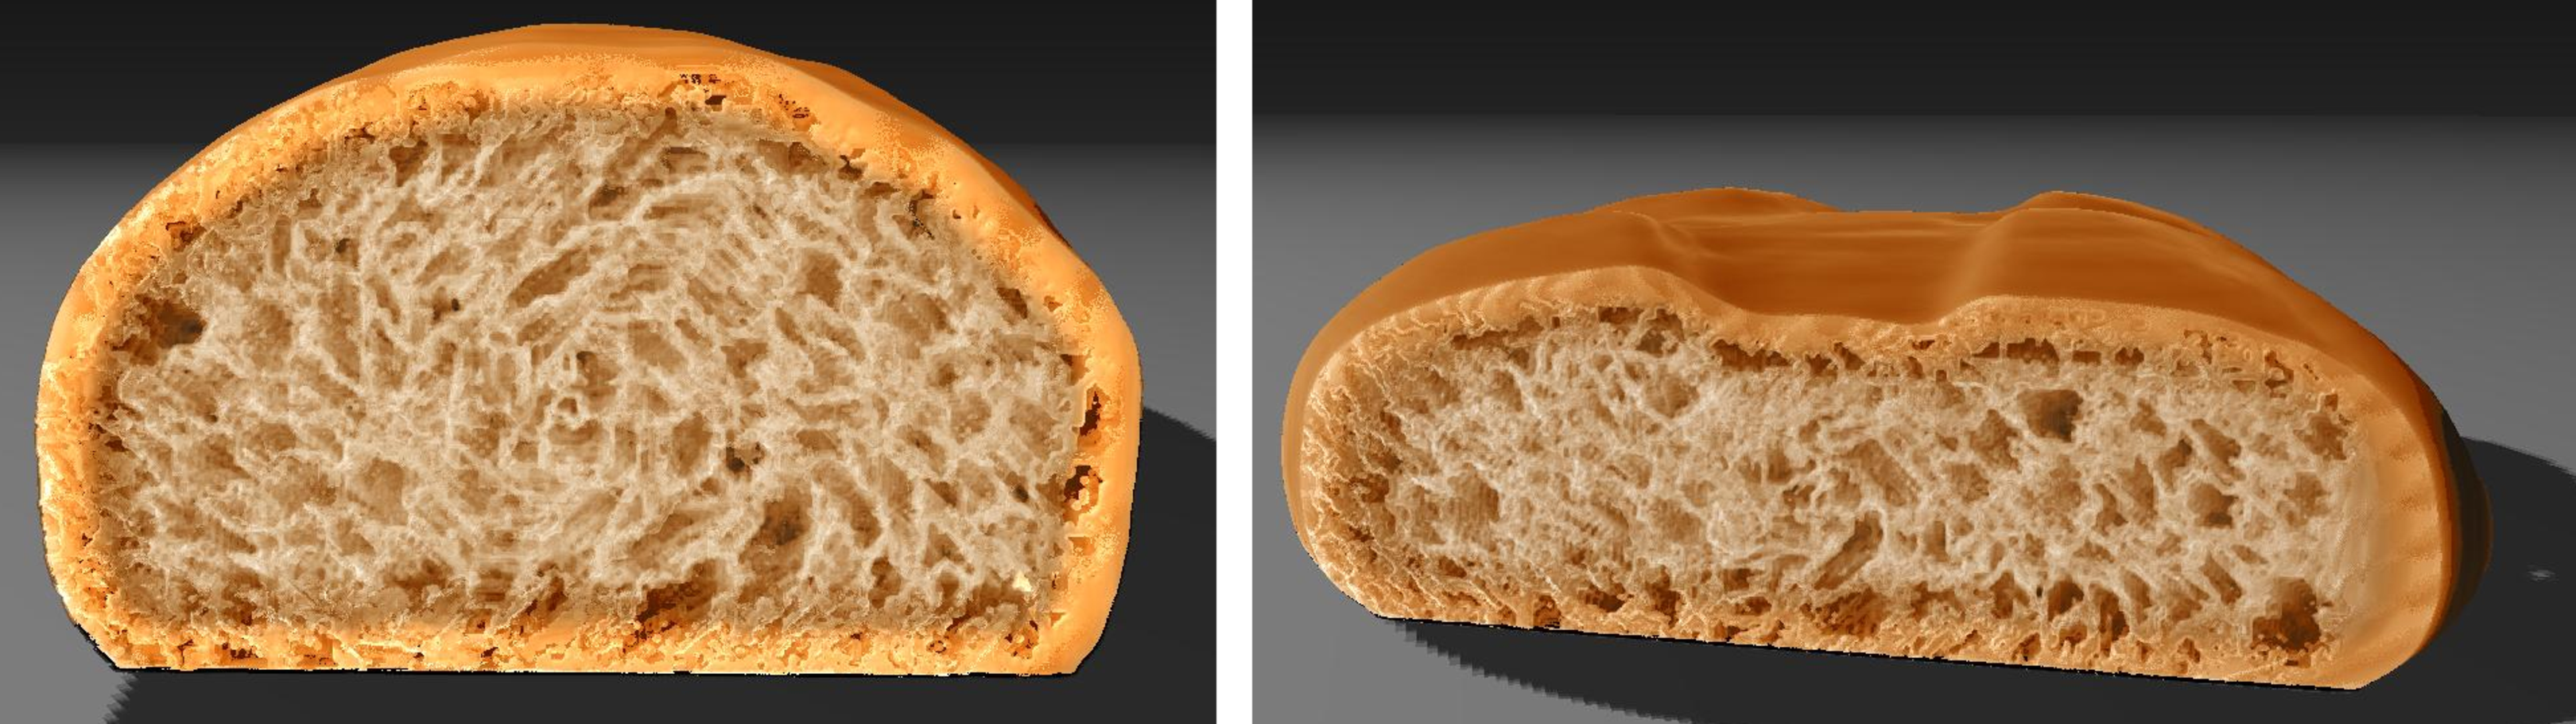
\includegraphics[width=10cm]{../figures/Fig11CAVW}}


Sistemas dinámicos adaptativos (dependiendo del ancho y alto del corte).

\centerline{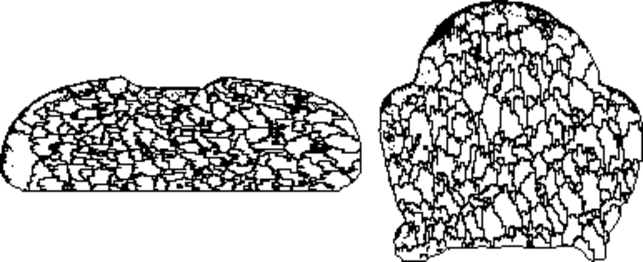
\includegraphics[width=7cm]{../figures/Fig6}}

\end{frame}

\begin{frame}{Resultados}
Parámetro {\em separación} = 2 entre partículas

\centerline{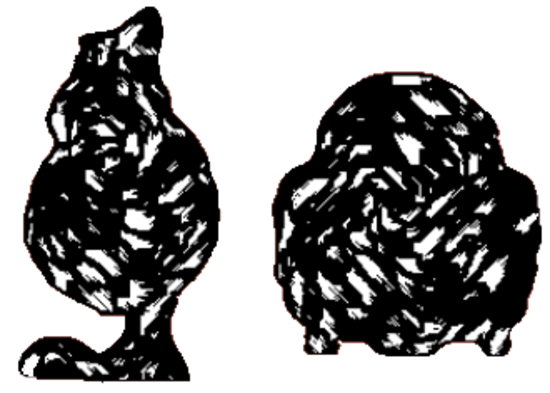
\includegraphics[width=8cm]{../figures/Fig7}}
\end{frame}

\begin{frame}{Renderizados}

\centerline{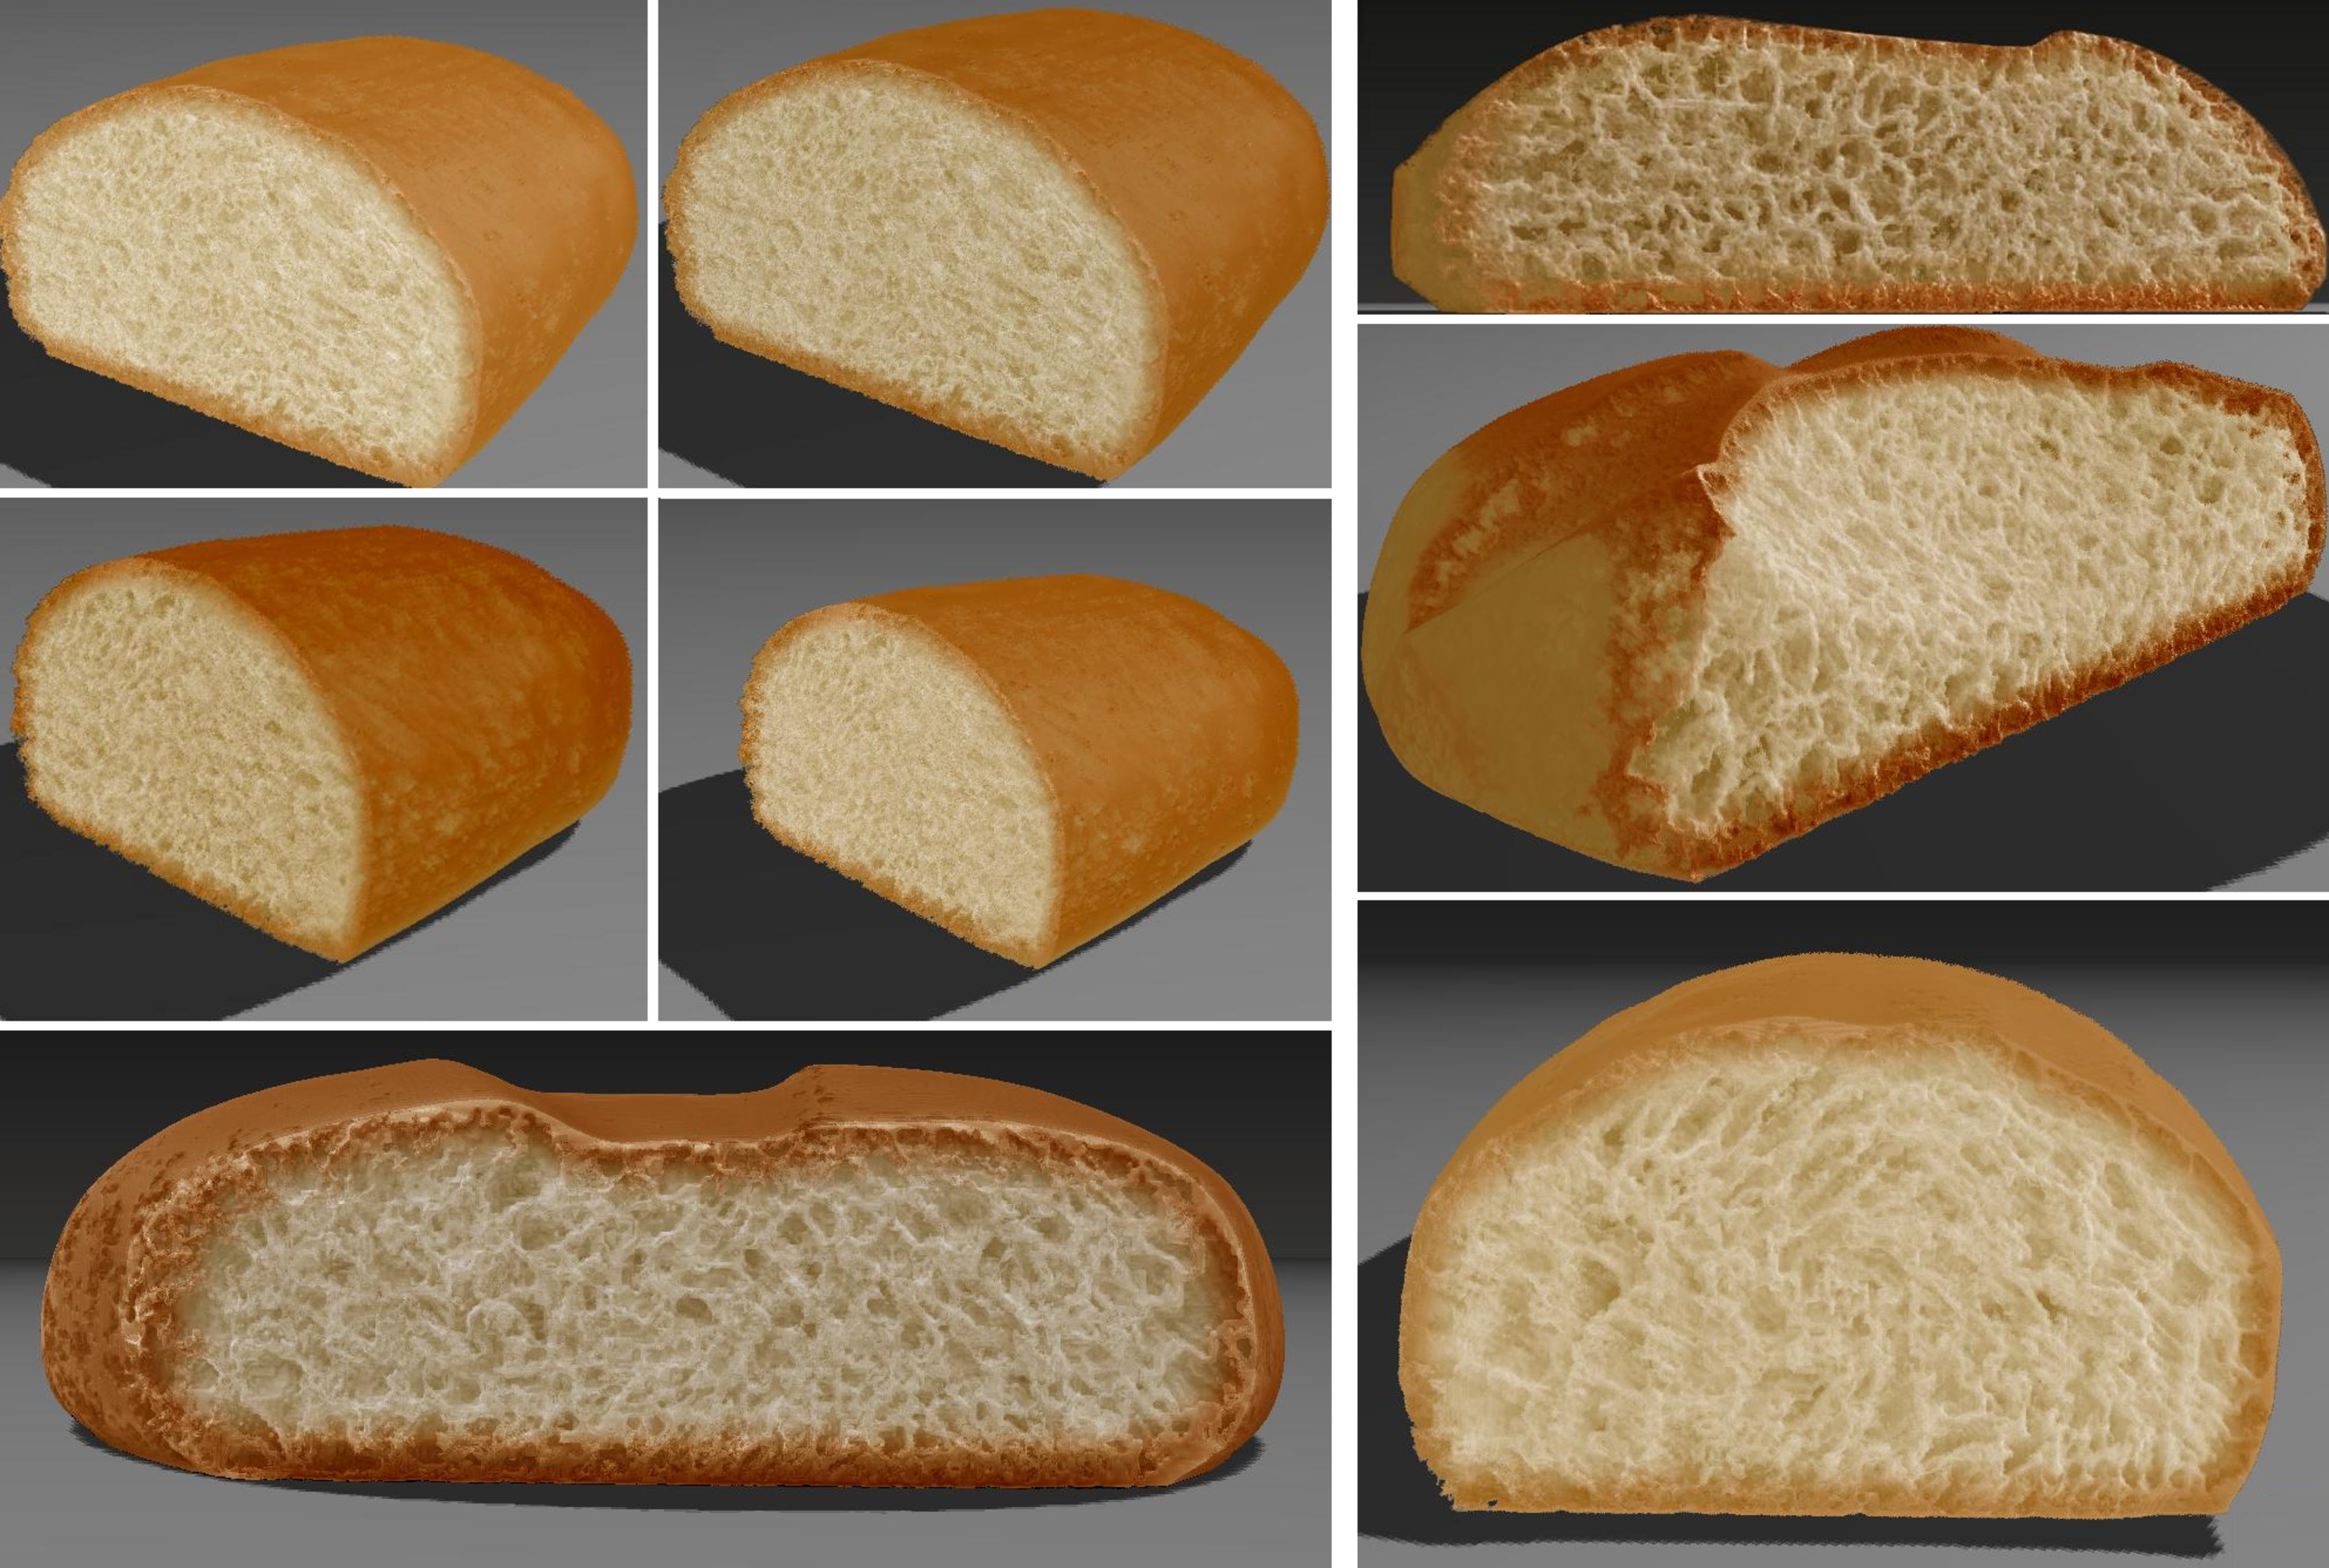
\includegraphics[width=10cm]{../figures/Fig12CAVW}}
\end{frame}

\begin{frame}{Esponjas}

\centerline{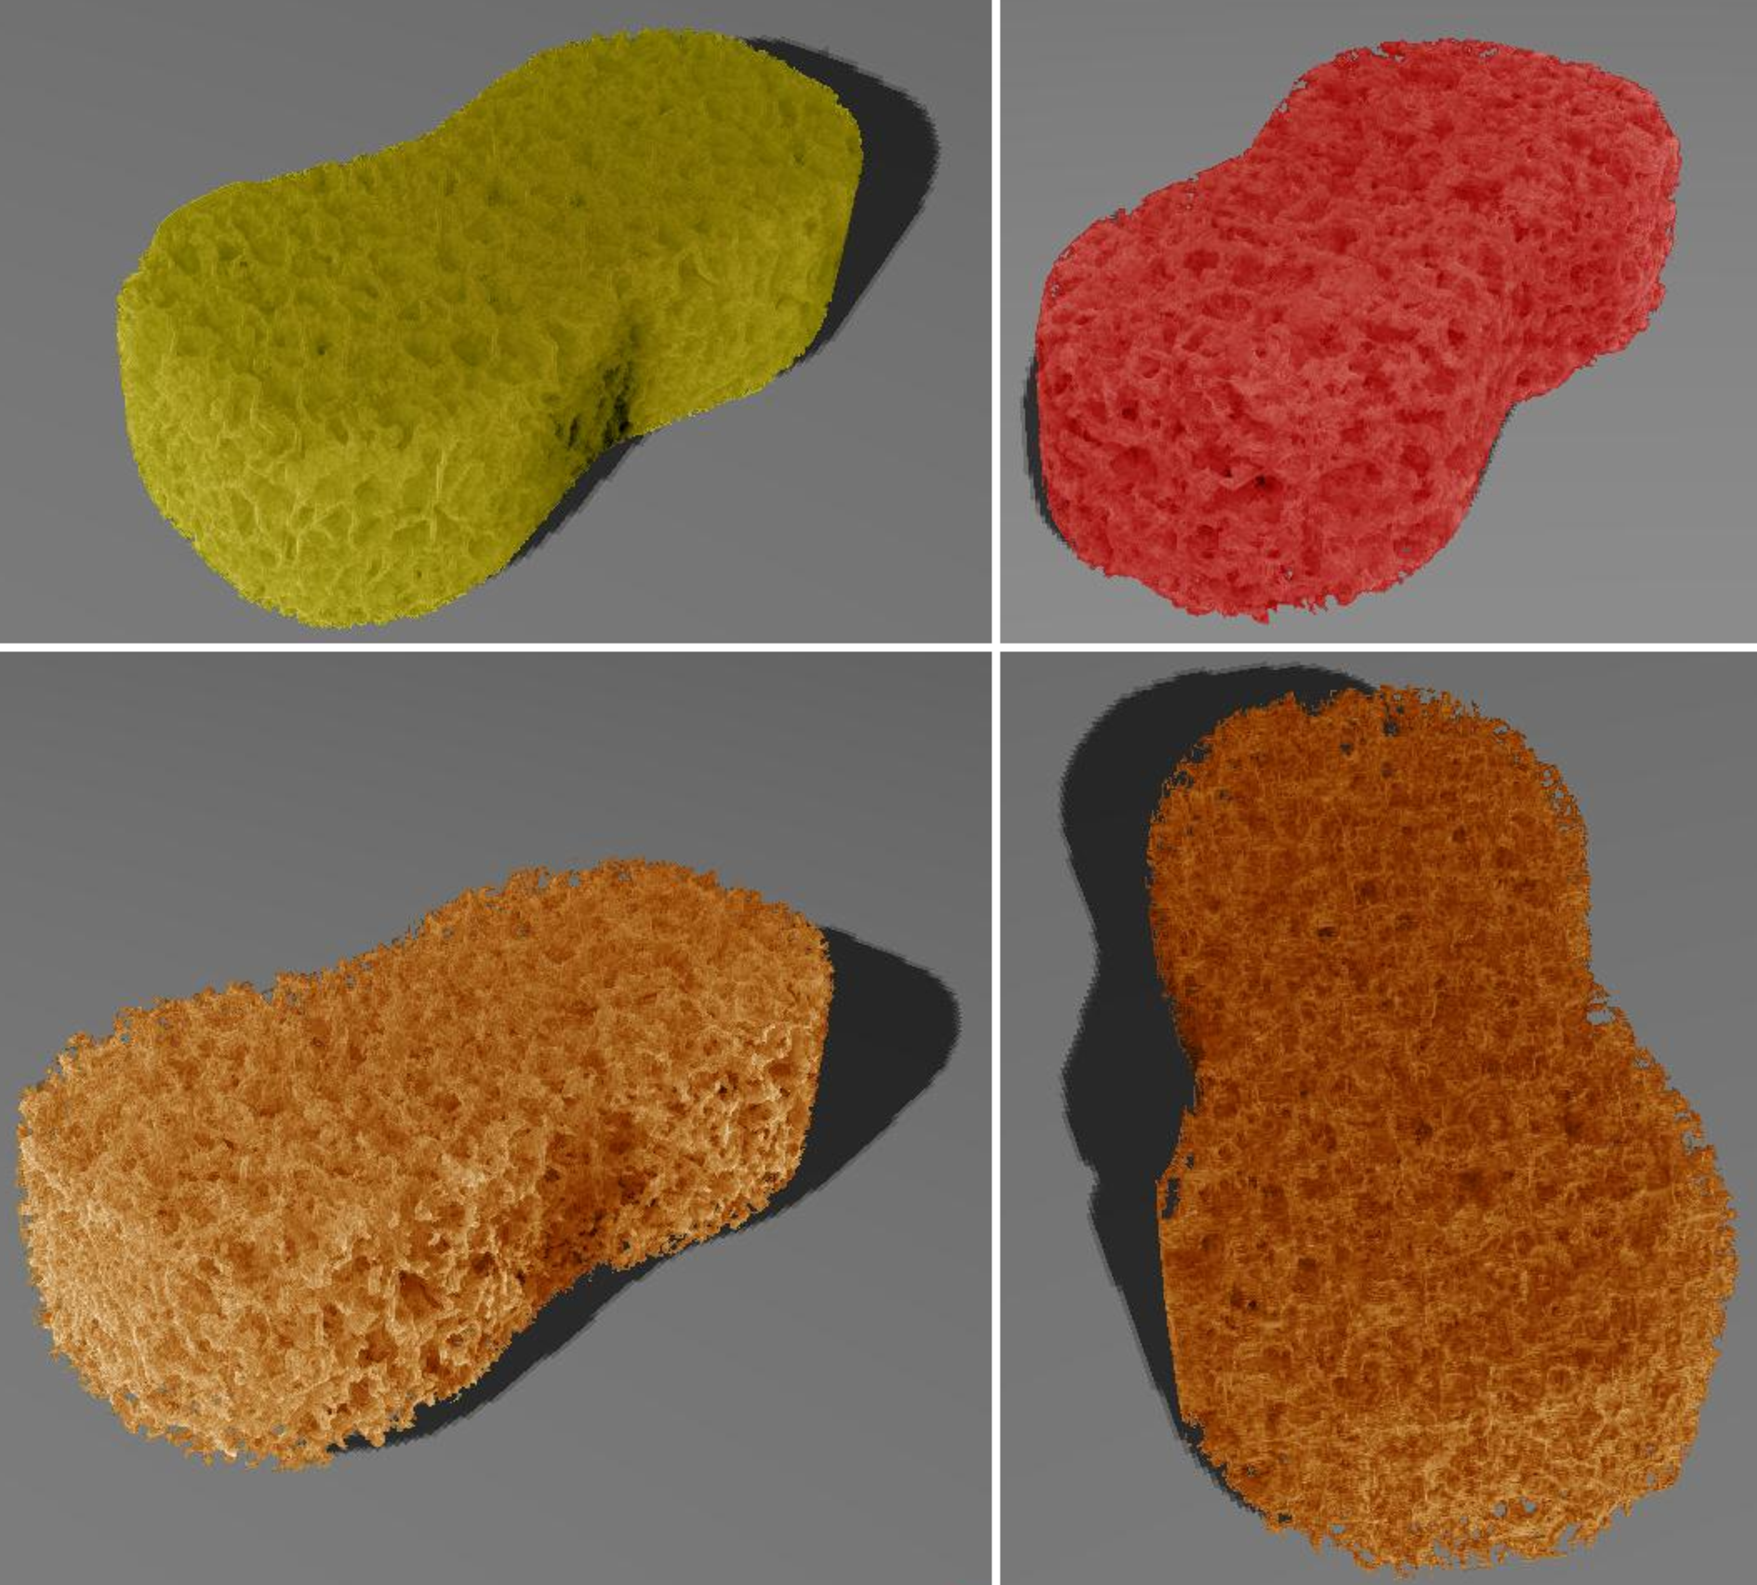
\includegraphics[width=7cm]{../figures/Fig13CAVW}}
\end{frame}

\begin{frame}{Piedras}

\centerline{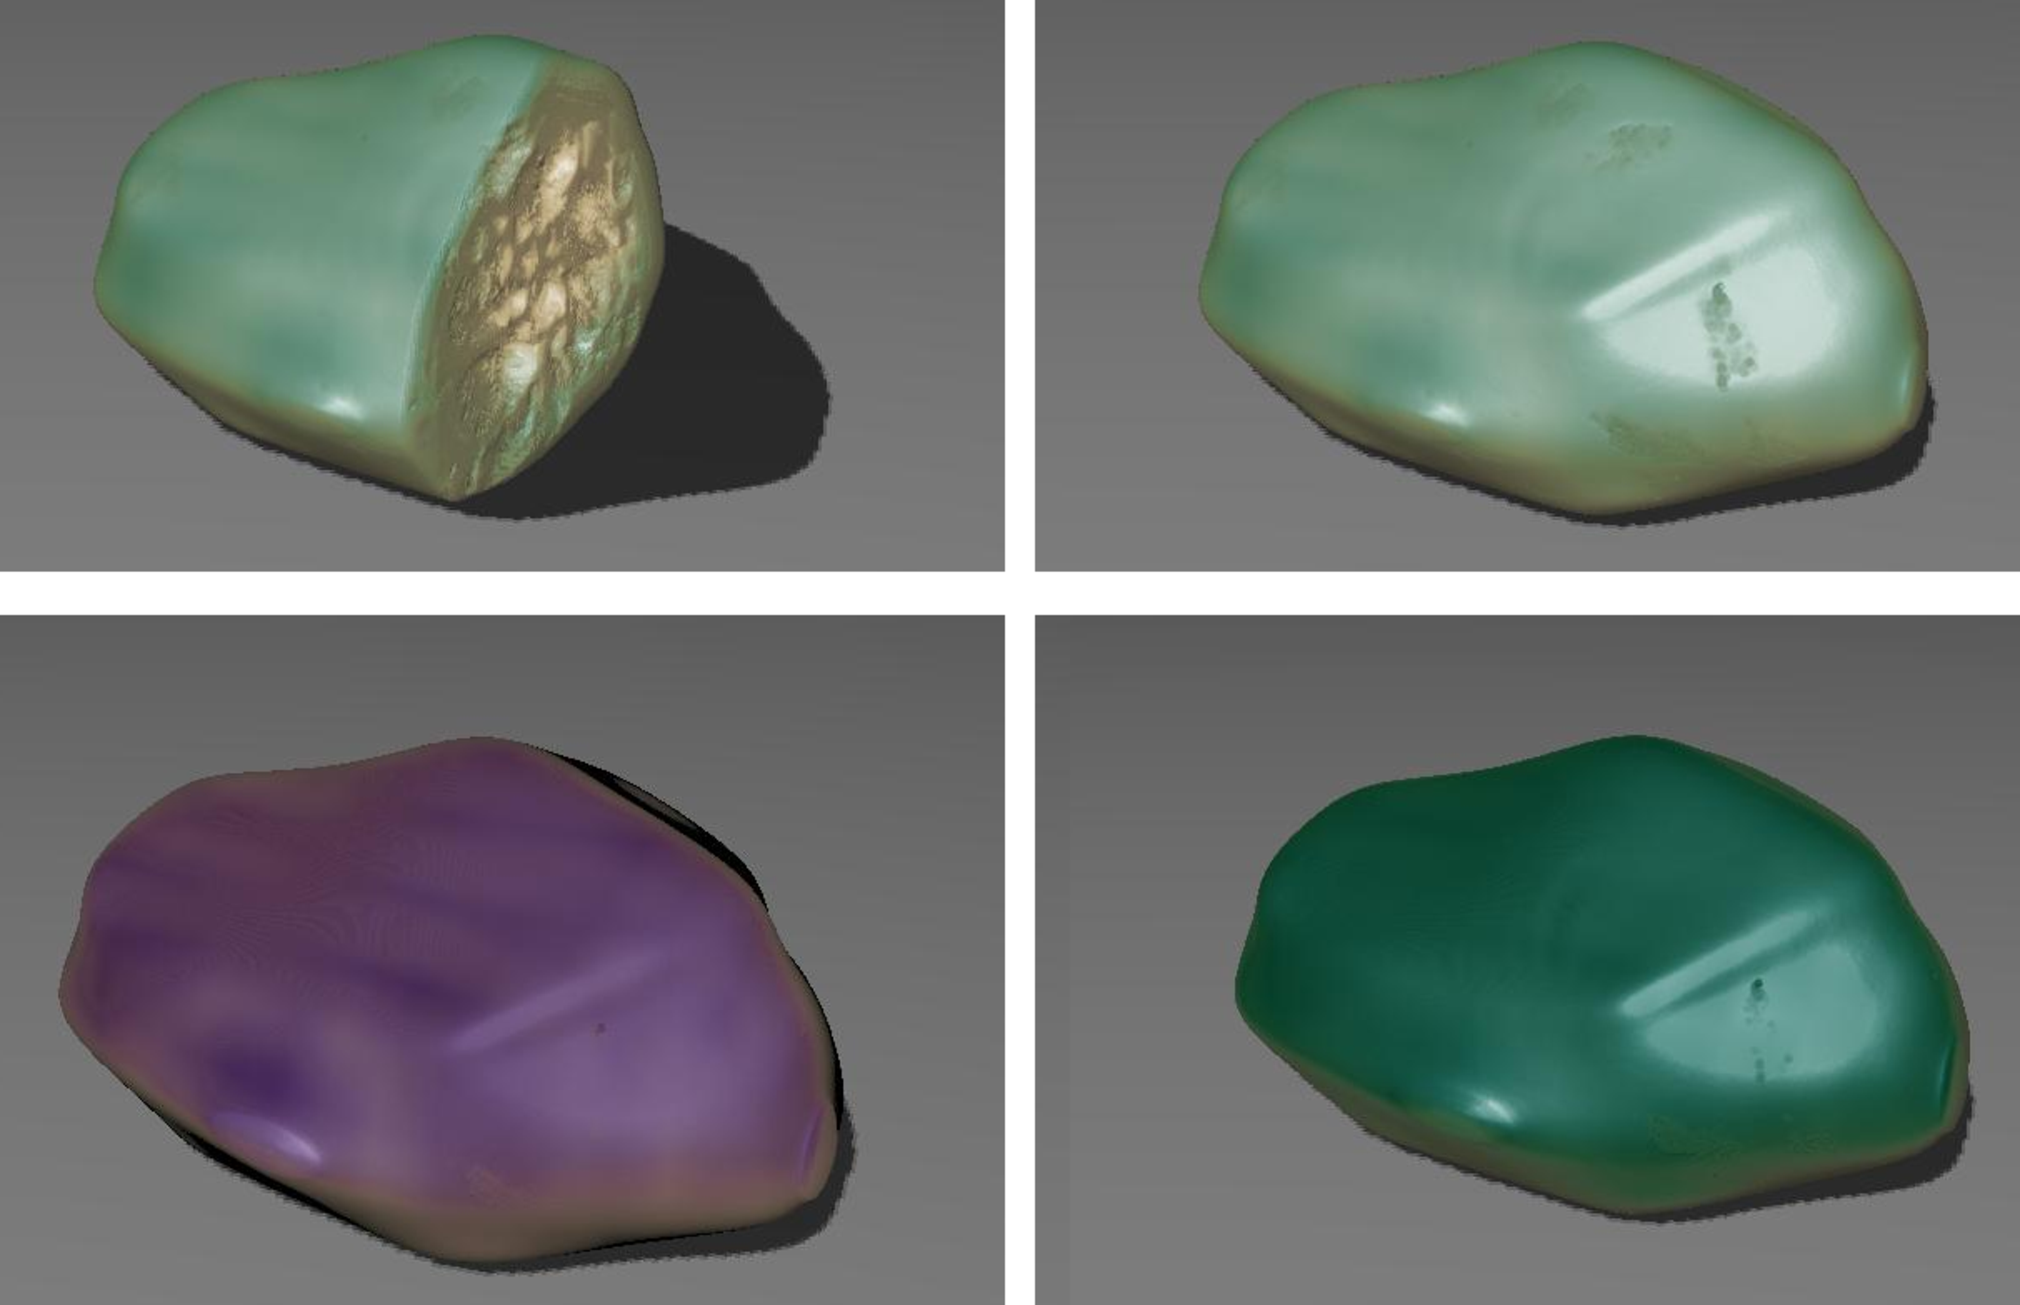
\includegraphics[width=9cm]{../figures/Fig14CAVW}}
\end{frame}

\begin{frame}{Conclusiones}
\begin{block}{}
\begin{itemize}
\item Algoritmo procedimental fenomenológico
\item Resultados adecuados para computación gráfica
\item Permite representar diversos materiales porosos
\item No requiere esfuerzo por parte del usuario

\item Dificultad al controlar los sistemas dinámicos
\end{itemize}
\end{block}
\end{frame}


\section[Modelado de Pan]{Modelado procedimental de pan inspirado en su proceso de formación}


\begin{frame}
\begin{block}{}
\begin{center}
\vspace{1cm}
\huge{Modelado procedimental de pan inspirado en su proceso de formación}
\vspace{1cm}
\end{center}
\end{block}
\end{frame}

\subsection{Modelado procedimental de pan inspirado en su proceso de formación}
\begin{frame}{Modelado procedimental de pan inspirado en su proceso de formación}
\begin{block}{}
\begin{itemize}
\item Debido a la complejidad del proceso, el mismo ha sido ignorado en gran medida en la literatura de computación gráfica.

\item Sin embargo, ha sido ampliamente estudiado en ingeniería de los alimentos.

\item No existe aún un modelo unificado. Los modelos existentes representan solamente subprocesos (cocción, leudado, formación de la corteza, etc.).

\item Es posible utilizar algunos de estos subprocesos para diseñar un algoritmo procedimental.
\end{itemize}
\end{block}
\end{frame}

\begin{frame}{Propuesta}
\centerline{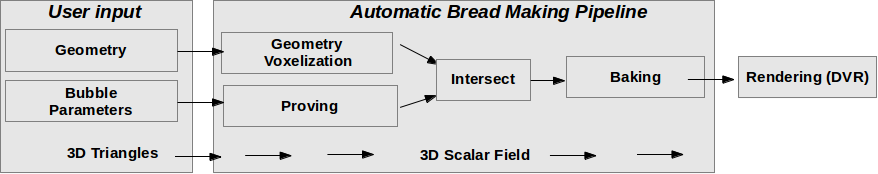
\includegraphics[width=12cm]{../figures/pipeline}}
\end{frame}

\begin{frame}{Leudado}
Se extraen esferas de un cubo, donde la cantidad de esferas $N(r)$ extraídas es inversamente proporcional al radio $r$ de la esfera, es decir, se utiliza la ley fractal

\begin{equation*}
N(r) = \frac{k}{r^{d}},
\end{equation*}

$k$ parámetro.

\centerline{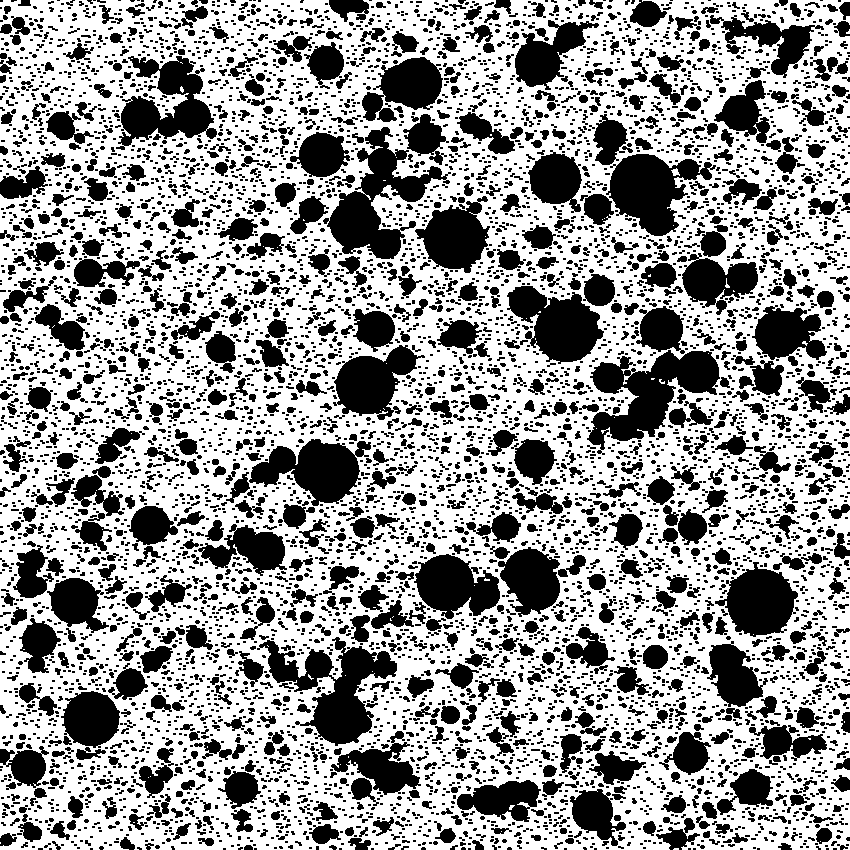
\includegraphics[height=4cm]{../figures/bubbles}}
\end{frame}

\begin{frame}
Si bien el proceso de generación utiliza una ley fractal, la intersección de las burbujas produce una estructura que no es necesariamente fractal, como se demostrará más adelante.

\vspace{1cm}

Es necesario disponer de las burbujas en una geometría de entrada, para esto, utilizar un enmascarado directo (multiplicación) produce resultados incorrectos:

\centerline{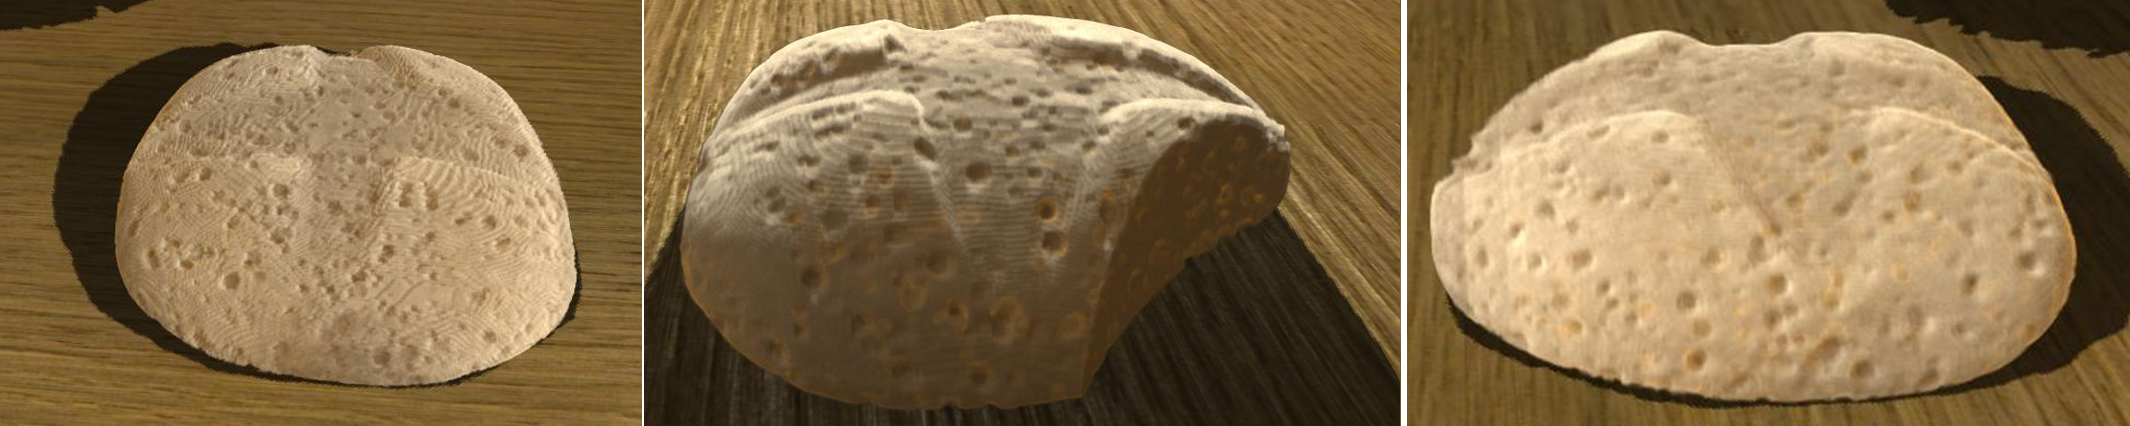
\includegraphics[width=8cm]{../figures/intersectProblem}}
\end{frame}

\begin{frame}
Se utiliza el mapa de distancias previamente discutido y un umbral, obteniéndose una región donde puede haber burbujas, permitiendo además obtener una corteza de ancho parametrizable.


\centerline{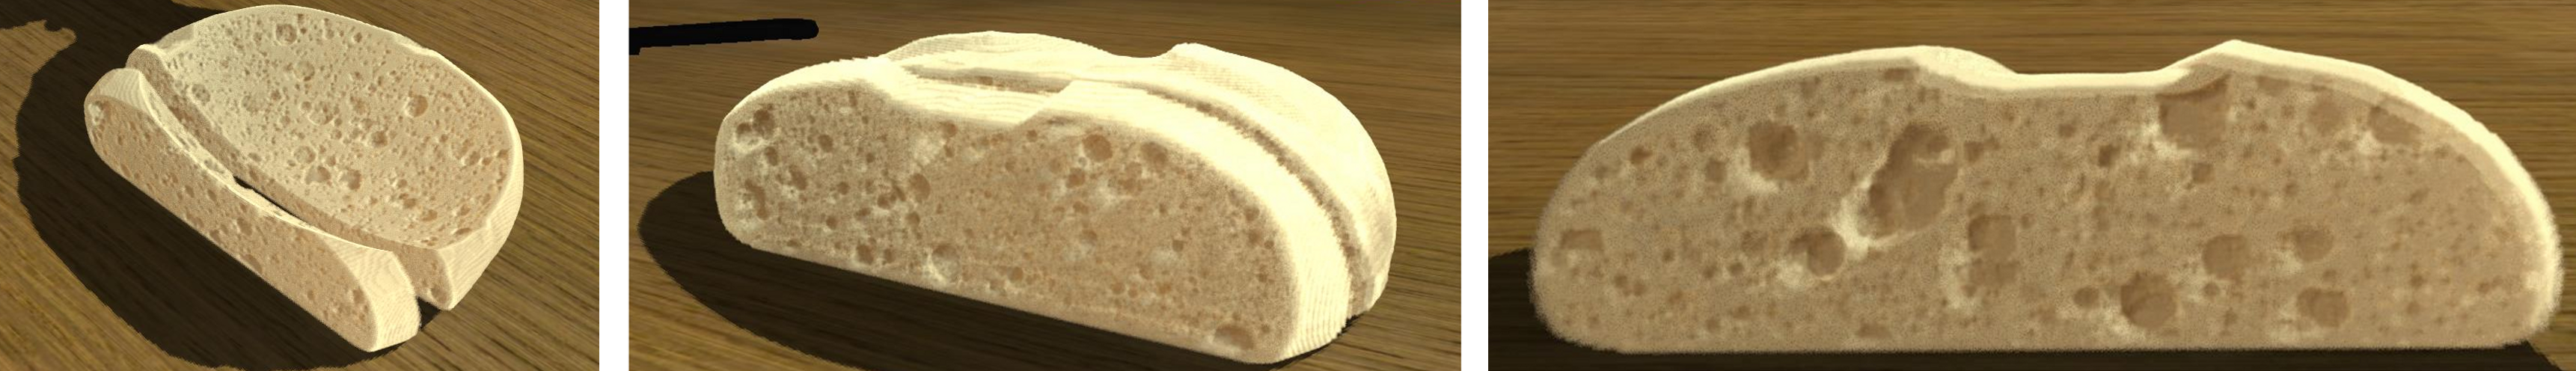
\includegraphics[width=10cm]{../figures/prebakebread}}
\centerline{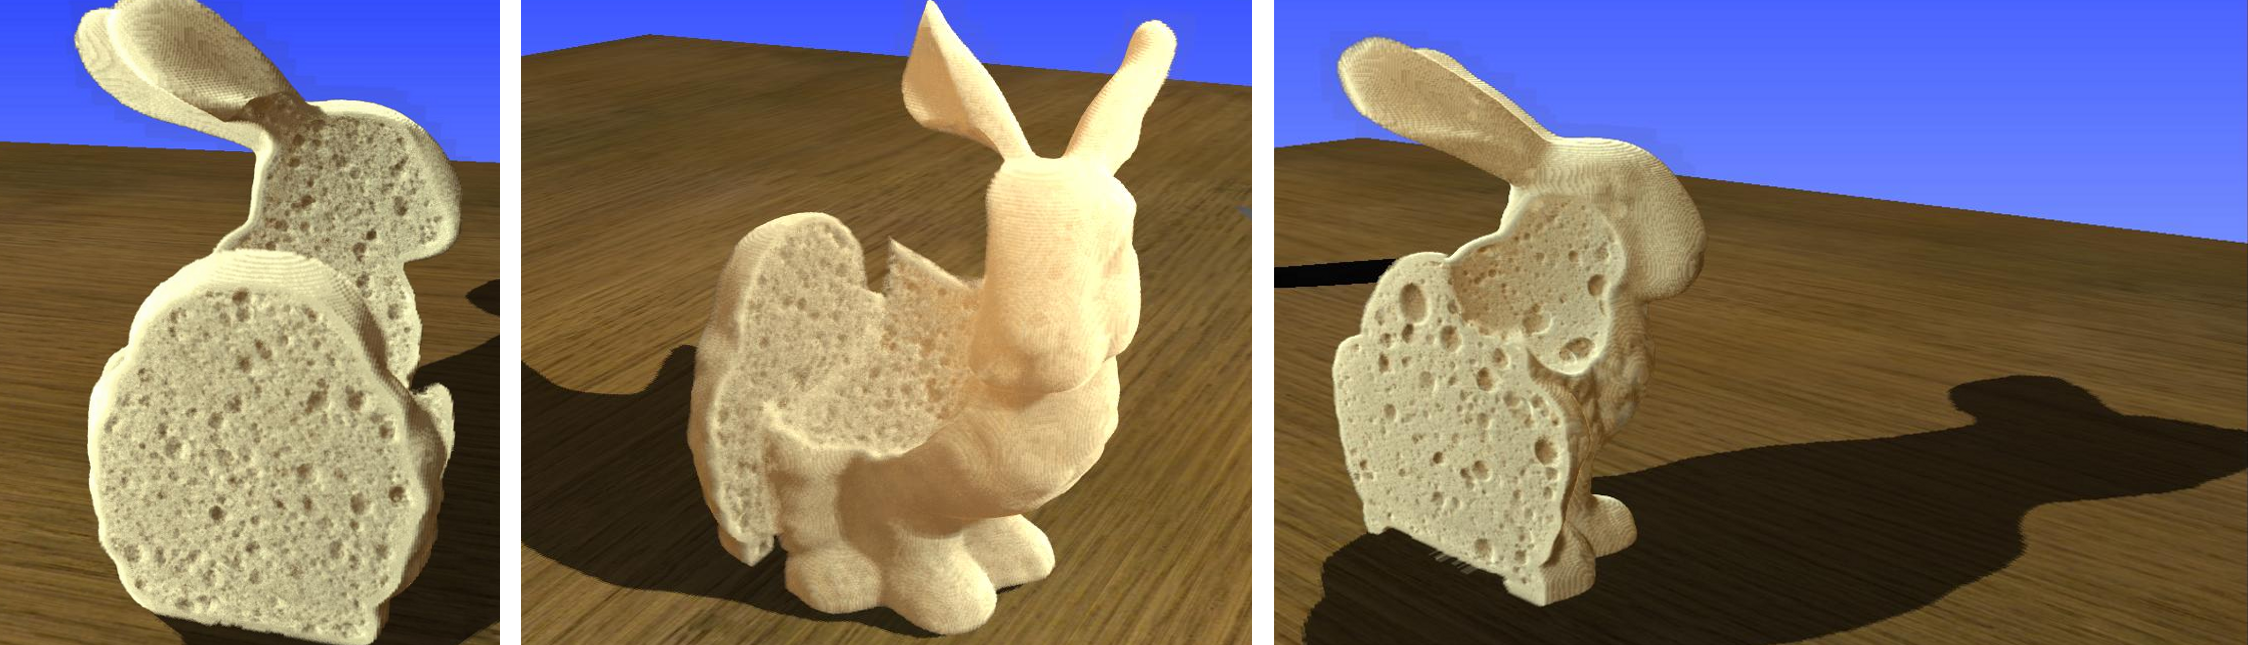
\includegraphics[width=10cm]{../figures/prebakebunny}}
\end{frame}

\subsection{Cocción}

\begin{frame}{Cocción}
Procesos durante la cocción:

\begin{itemize}
\item Transferencia de calor y masa
\item Crecimiento de las burbujas
\item Deformación de la masa original
\item Formación de la corteza
\item Reacciones químicas
\end{itemize}

En nuestro caso, debe atenderse especialmente al efecto de dichos procesos sobre la \textbf{apariencia}.

\end{frame}

\begin{frame}{Cocción}
Modelo unidimensional

\begin{equation}
\label{Eq:heat}
\frac{\partial T}{\partial t} = \frac{1}{\rho C_{p}} \frac{\partial}{\partial x} \left ( k \frac{\partial T}{\partial x} \right ) + \frac{\lambda}{C_{p}} \frac{\partial W}{\partial t}+\frac{\lambda W}{ \rho C_{p} }\frac{\partial \rho}{\partial t},
\end{equation}
%
\noindent donde

$T$ temperatura, $x$ es la coordenada radial, $t$ tiempo, $C_{p}$ calor específico, $\rho$ densidad, $k$ conductividad térmica, $\lambda$ calor latente de la evaporación de agua, y $W(x,t)$ contenido de agua líquida.

Condiciones iniciales:
\begin{align*}
T(x,0) &= T_{0}(x), 0\le x \le L/2,
\end{align*}

\end{frame}

\begin{frame}{Cocción}
Condiciones de borde (continuidad y suavidad)
\begin{align*}
\left ( \frac{\partial T}{\partial x} \right )_{x=L/2} &= 0 , t > 0 \\
-k \left ( \frac{\partial T}{\partial x} \right )_{x=0} &= h_{r}(T_{r}-T_{s}) + h_{c}(T_{air}-T_{s}) - \lambda \rho D_{w} \left (\frac{\partial W}{\partial x} \right )_{x=0}
\end{align*}
%

\end{frame}

\begin{frame}
Horno a una temperatura típica (por defecto utilizamos $210^{\circ}C$) y discretiza el tiempo en intervalos $\Delta t = 30s$.


De la simulación se obtiene un arreglo unidimensional $Temp$, de tamaño $N_{grid}$, compuesto por valores de temperatura.

Luego, obtenemos una distribución 3D de la temperatura
\begin{equation*}
\displaystyle R_{vol}[x,y,z] = Temp[ round( DF_{M}[x,y,z] ) ], 
\end{equation*}

$DF_{M}[(x,y,z)] = 0 \rightarrow$ contorno, $Temp[0] \rightarrow R_{vol}[(x,y,z)]$.
$DF_{M}[(x,y,z)] > 0 \rightarrow$ interior, $<$ T  $\rightarrow R_{vol}[(x,y,z)]$, .

\centerline{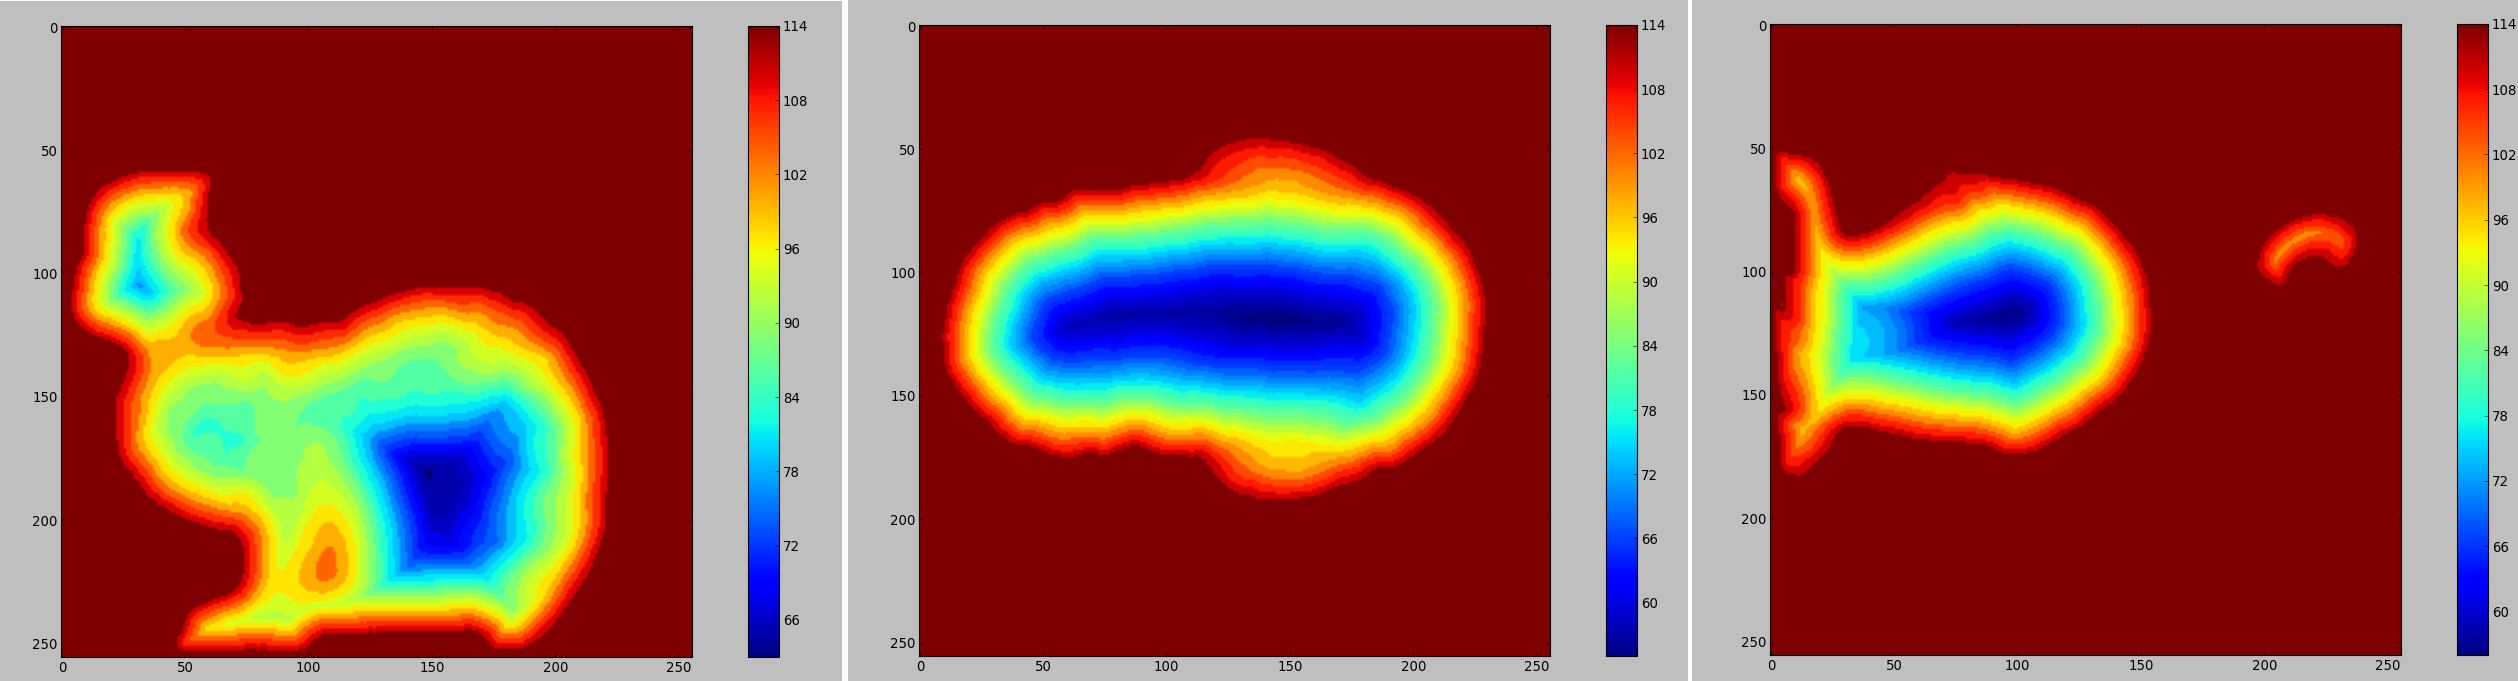
\includegraphics[width=8cm]{../figures/tempsbunny}}
\end{frame}

\begin{frame}{Deformación por Temperatura}

Utilizamos una operación de warping, deformando las burbujas de acuerdo a la temperatura, en tres dimensiones, reemplazando así los sistemas dinámicos de la sección anterior.

Se aplica un filtrado gaussiano al gradiente de $R_{vol}$, obteniendo $g'$

\begin{align*}
\displaystyle
[x,y,z] = [u,v,w] + p\, g'[u,v,w],
\end{align*}

Efecto de $p = 5,10,15$, respectivamente
\centerline{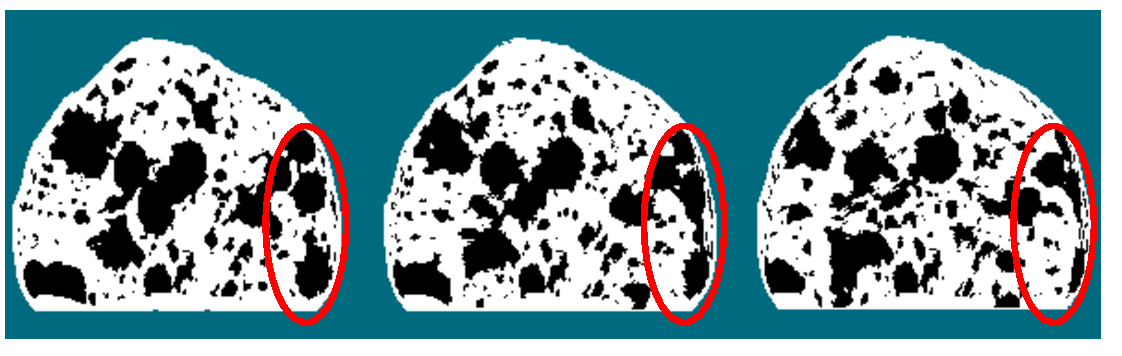
\includegraphics[width=11cm]{../figures/parameterp}}

\end{frame}

\begin{frame}{Levantamiento de la masa}

Una segunda operación simula el levantamiento de la masa, basado en la distribución de burbujas durante el leudado.
\begin{equation*}
P[x,y,z] = max \bigg\{r\bigg\}
\end{equation*}

El parámetro $p$ se trata localmente, entonces $p = P[u,v,w],$

\begin{equation*}
[r,s,t] = [u,v,w] + P[u,v,w] \, g'[u,v,w],
\end{equation*}

%\noindent donde $[u,v,w]$ es la entrada original, y $[r,s,t]$ es la coordenada deformada.


Finalmente, se escala la textura de acuerdo a la distribución de burbujas,


\begin{equation}
[x,y,z] = [r,s,t]\, S \, P[r,s,t],
\end{equation}

\noindent donde $[x,y,z]$ es la entrada final, luego de la deformación inducida por el crecimiento.

\end{frame}

\begin{frame}{Resultados}

\centerline{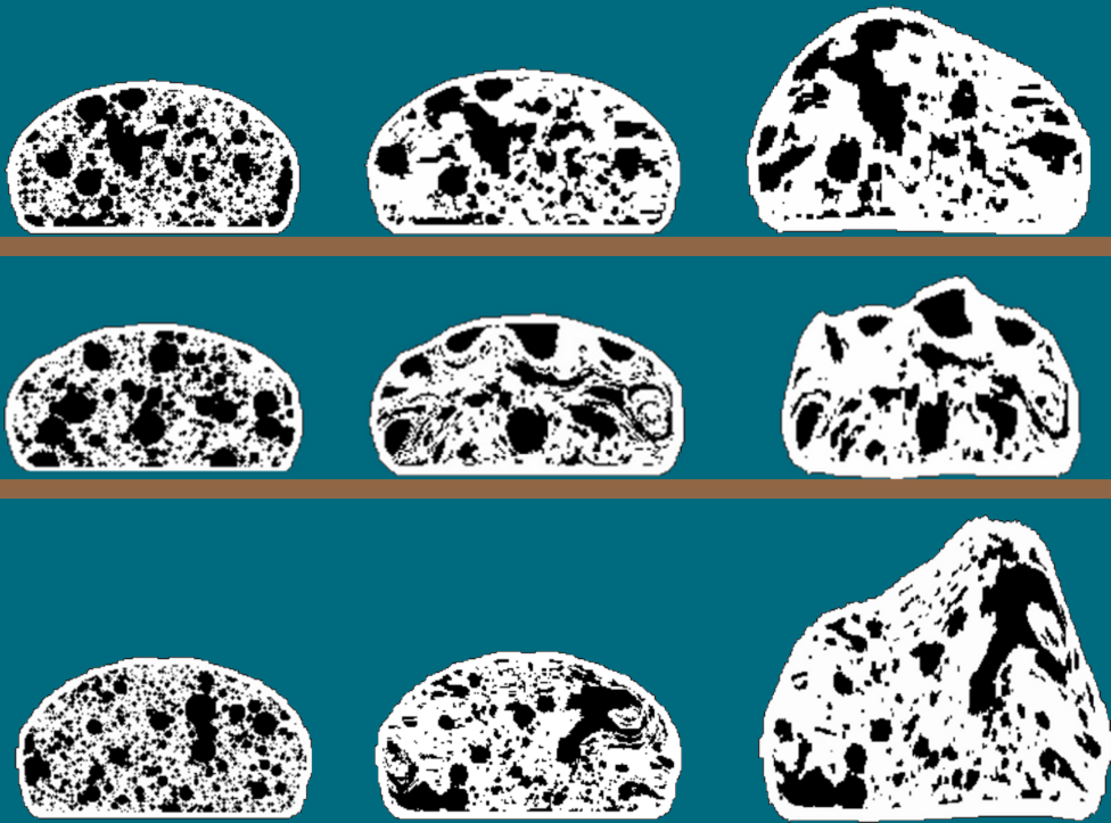
\includegraphics[width=9cm]{../figures/Fig9}}

\end{frame}

\subsection{Corteza}

\begin{frame}{Corteza}
Tomamos colores CIELab de muestras reales, reportadas por Purlis et. al. (2009).

$$L = 40 \rightarrow \text{máxima cocción}$$

$$L = 90 \rightarrow \text{sin cocción}$$

\centerline{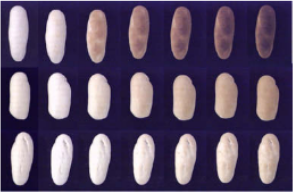
\includegraphics[width=4cm]{../figures/browning}}

\end{frame}

\begin{frame}

Los valores de los canales $a$ y $b$ no están reportados. A partir de fotografías se observa que varian suavemente al cambiar $L$.

{\em \textbf{Densidad} de la corteza}: $N_{v} / W_{size},$ donde $N_{v}$ número de voxels $= 1$ en una ventana en el entorno de la posición, y $W_{size}$ número de voxels en esa ventana.

Los colores se distribuyen de acuerdo al valor de $L$. $<$ masa $\Rightarrow < L$.

\end{frame}


\subsection{Resultados}

\begin{frame}{Resultados}

\centerline{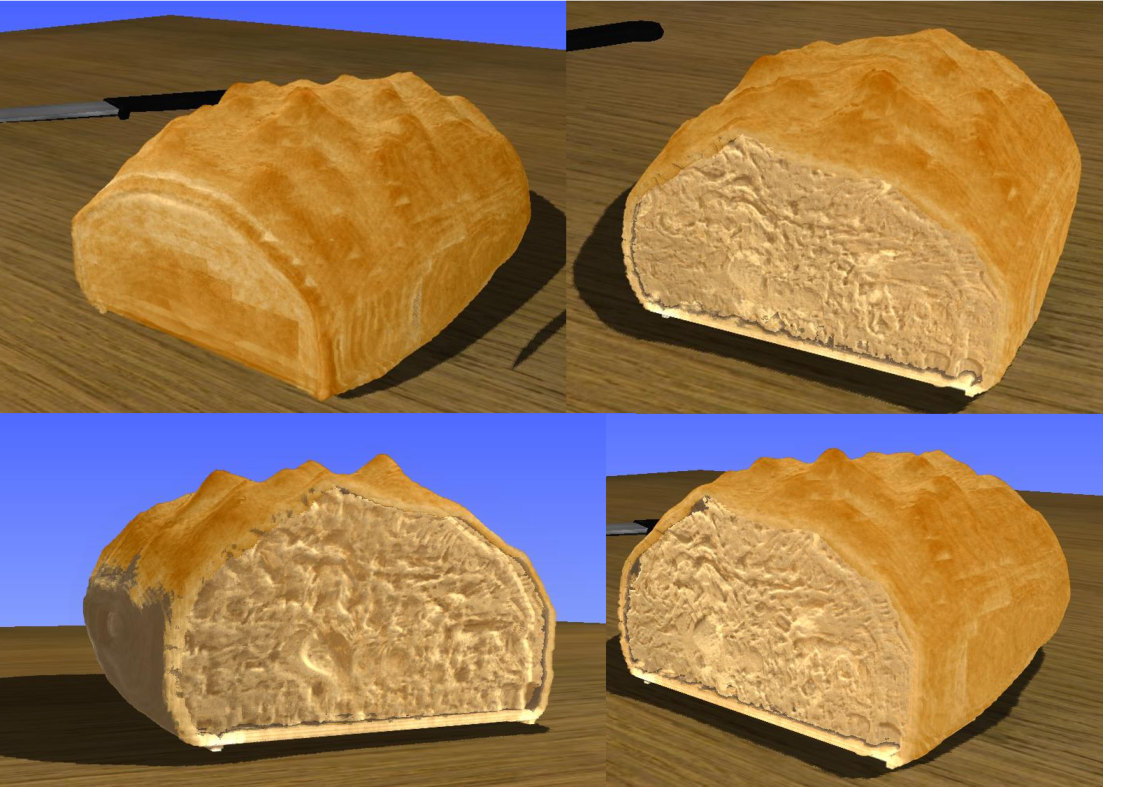
\includegraphics[width=9cm]{../figures/Fig11}}

$S$ con valores aleatorios en cada punto, picos visibles en la corteza.

\end{frame}

\begin{frame}{Resultados}

\centerline{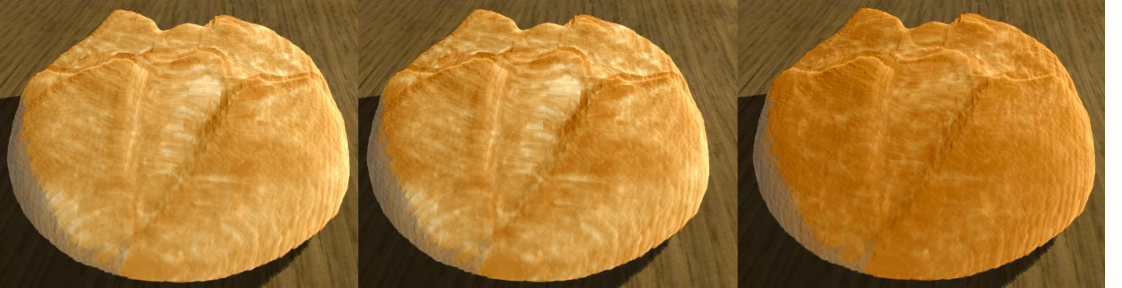
\includegraphics[width=12cm]{../figures/Fig13}}
Cortezas con diferentes historias de cocción. De izquierda a derecha, se decrementa el valor máximo admitido para el canal $L$.

\end{frame}

\begin{frame}{Resultados}
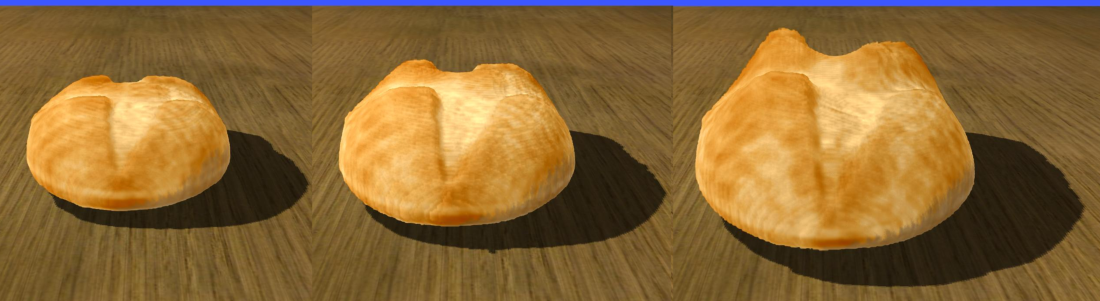
\includegraphics[width=11cm]{../figures/Fig14}

Panes luego de la cocción mostrando diferentes crecimientos. De izquierda a derecha se incrementa el parámetro $S$.

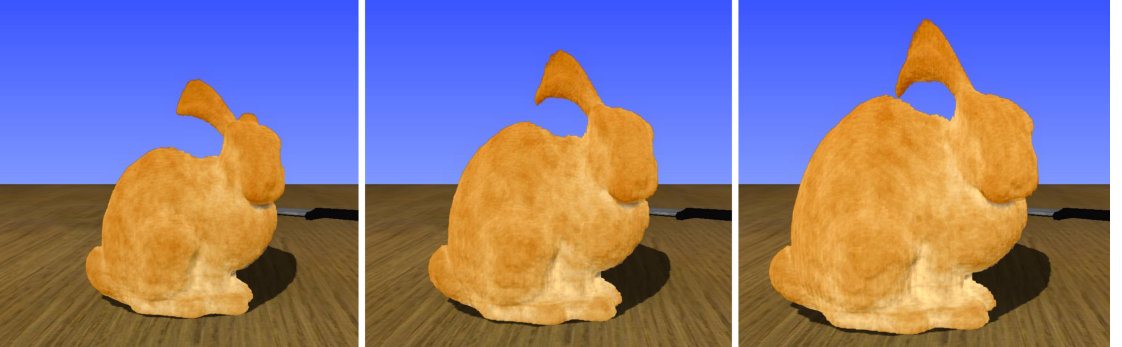
\includegraphics[width=9cm]{../figures/Fig15}


\end{frame}

\begin{frame}{Tiempos de Cómputo}

\begin{table}[h!]
       % Give a unique label
% For LaTeX tables use
\begin{tabular}{lllll}
\hline\noalign{\smallskip}
Resolución de la Textura Volumétrica & $256^{3}$ & $384^{3}$  & $512^{3}$ \\
\noalign{\smallskip}\hline\noalign{\smallskip}
Leudado & 3.62 & 12.07 & 31.29 \\
Intersección & 8 & 10.27 & 14.97 \\
Transformación de Distancia & 7 & 23.73 & 56 \\
Cocción  & 49.81 & 144.69 & 313.7 \\
\hline\noalign{\smallskip}
Total & 68.43 & 190.76 & 415.96 \\
%Rendering & 1s & 4s & 0\% \\
\noalign{\smallskip}\hline
\end{tabular}
\caption{Tiempos de cómputo típicos en de las distintas etapas de la fabricación sintética de pan, expresados en segundos.}
\label{tab:computingtimes}
\end{table}
\end{frame}

\begin{frame}{Conclusiones}
\begin{block}{}
\begin{itemize}
\item Modelo \textbf{inspirado} físicamente
\item Elimina decisiones ad-hoc
\item Se simula cocción, levantamiento de la masa, etc.
\item Permite obtener imágenes en sucesivas etapas del proceso de formación
\end{itemize}
\end{block}
\end{frame}

\section{Renderización}


\begin{frame}
\begin{block}{}
\begin{center}
\vspace{1cm}
\huge{Renderización}
\vspace{1cm}
\end{center}
\end{block}
\end{frame}


\subsection{Renderización}

\begin{frame}{Renderización}

Muchas técnicas de renderizado utilizan \textbf{mallas} para computar los resultados.
Esto es, la geometría se representa por vértices, y conexiones entre ellos, formando triángulos u otras figuras geométricas.

\ \\

En nuestro caso, contamos con una \textbf{textura volumétrica}, por lo tanto proponemos utilizar Renderizado Directo de Volúmenes para evitar la construcción de una malla.

Además, de esta forma será posible obtener cortes arbitrarios del material.

\end{frame}

\begin{frame}{DVR}
DVR aproxima la Ecuación del Transporte Radiativo (RTE).

Se computa un \textbf{rayo} para cada pixel, desde la pantalla al objeto. El algoritmo computa el cambio de radiancia a lo largo del medio.


\centerline{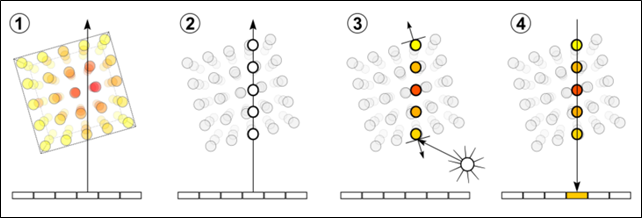
\includegraphics[width=9cm]{../figures/dvr}}

Para obtener resultados en tiempo real, tomamos una versión simplificada de la RTE, teniendo en cuenta solamente la transmitancia.
\end{frame}

\begin{frame}{Renderización}


Sea el \textbf{coeficiente de absorción} $ = \int_{p_i}^{p_j} k_a(t) \, dt$  $ = \tau_{(p_i, p_j)}$.


Entonces la \textbf{Transmitancia} es la cantidad de luz que \texttt{atraviesa} un segmento del volumen:

\begin{equation*}
  T(p_i,p_j) = e^{-\tau_{(p_i, p_j)}}.
\end{equation*}


\centerline{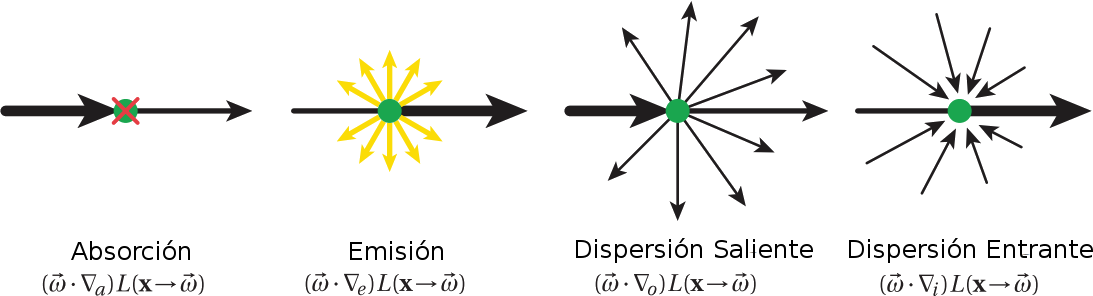
\includegraphics[scale = 0.25]{../figures/fenomenosrte}}


\end{frame}

\begin{frame}{Radiancia}


\textbf{Radiancia}: cantidad de luz que pasa o es emitida por un medio.

\begin{equation*}
  L(p_n) = L_b \ e^{-\tau(p_0, p_n)} + \int_{p_0}^{p_n} \rho \ e^{-\tau(t,p_n)} \, dt.
\end{equation*}

(Radiancia de fondo $+$ Radiancia del medio)

%La implementación reemplazará la integral por una suma,

\begin{equation*}
  L(p_n) = L_b \ e^{-\tau(p_0, p_n)} + \sum_{p_0}^{p_n} \rho \ e^{-\tau(p_i,p_n)}.
\end{equation*}


\end{frame}


\begin{frame}{DVR en GPU}

\begin{itemize}
\item Computamos un rayo principal desde la cámara hacia el volumen
\item Cada paso del rayo origina un rayo secundario, computando la transmitancia desde la posición actual hacia la luz, produciendo sombras
\end{itemize}

\centerline{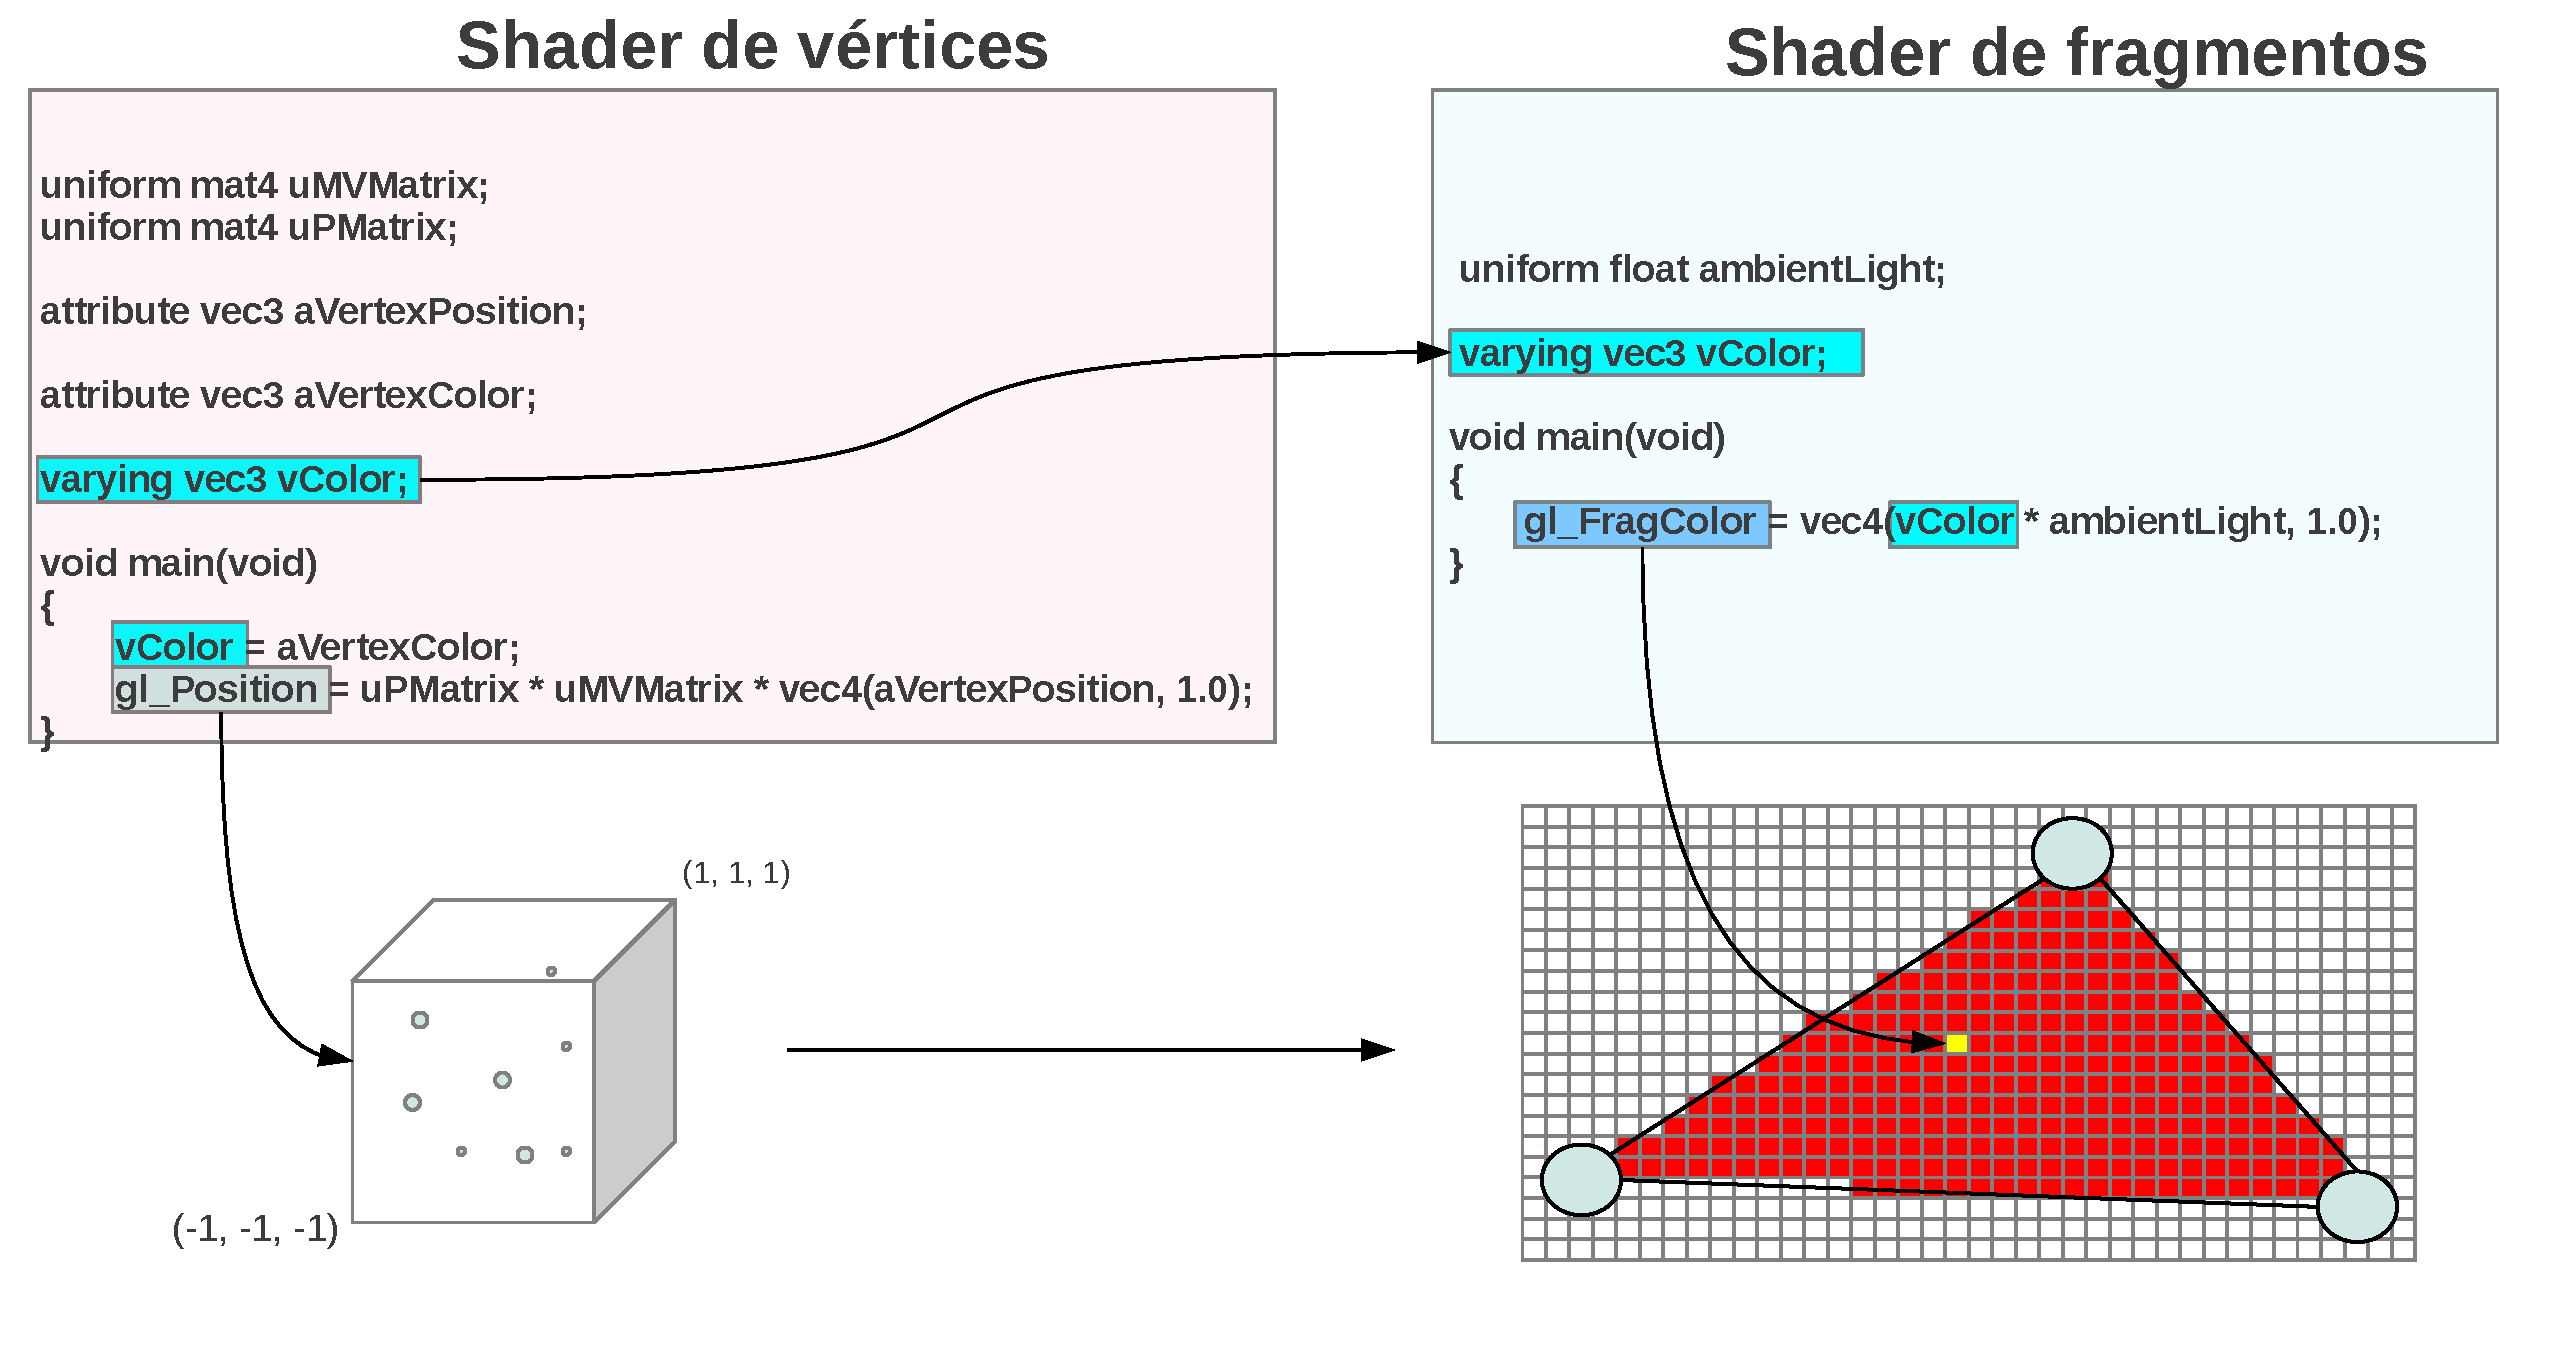
\includegraphics[width=4cm]{../figures/fragmentshader}}

\end{frame}

\begin{frame}
Esto se implementa en la GPU, en el denominado \textbf{fragment shader}, el cual es el paso del \textbf{pipeline gráfico} que opera sobre fragmentos (píxeles).

\centerline{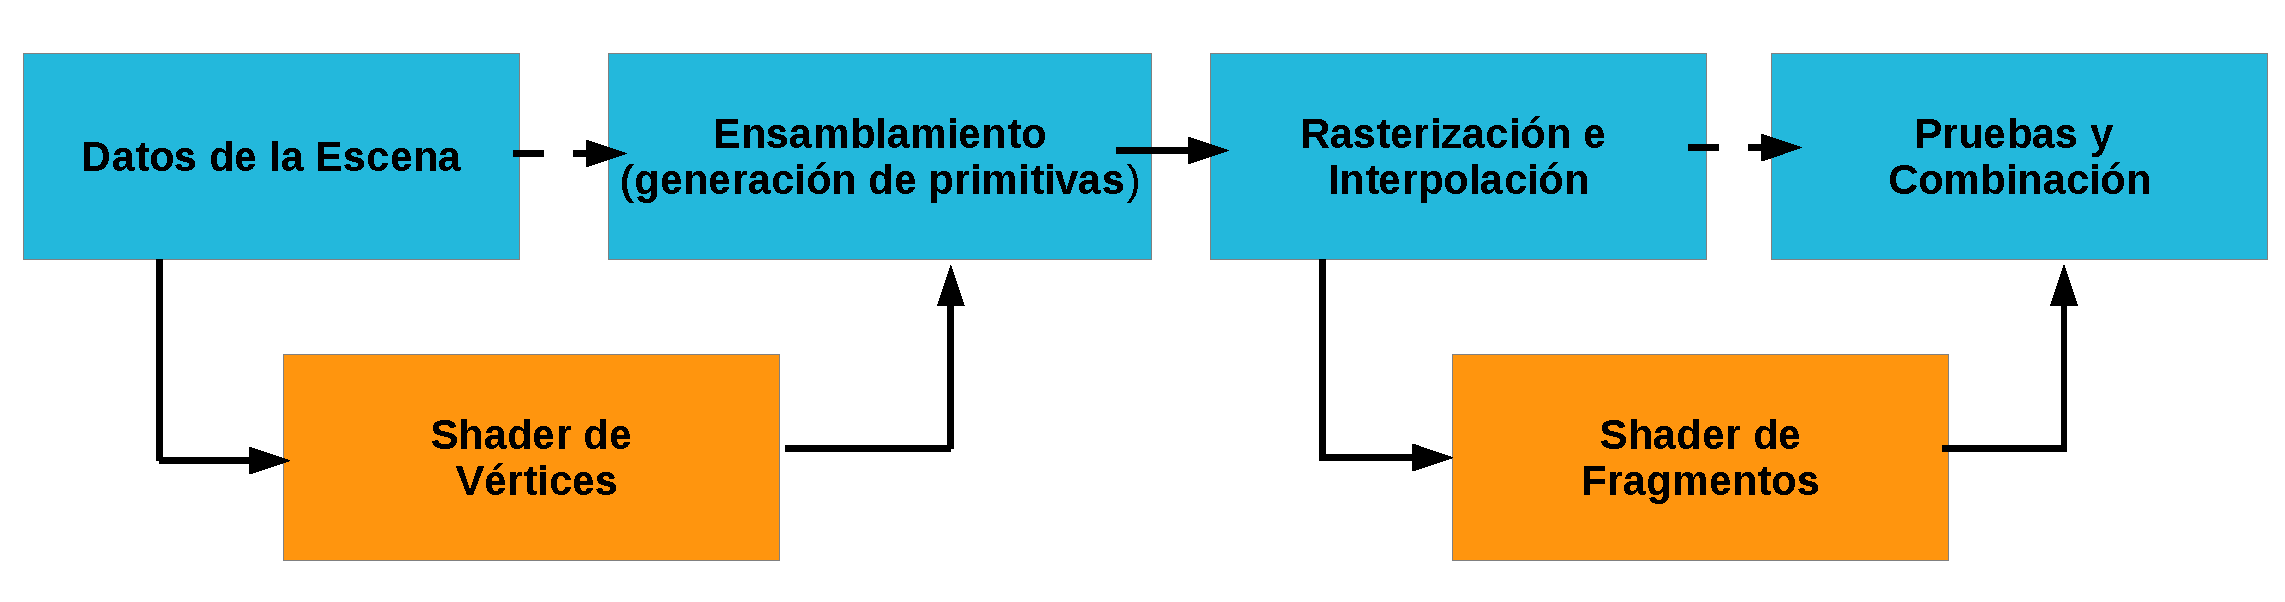
\includegraphics[width=13cm]{../figures/pipelinegrafico}}
\end{frame}

\begin{frame}{Tiempos de Cómputo}

\begin{table}[htb]
\centering
%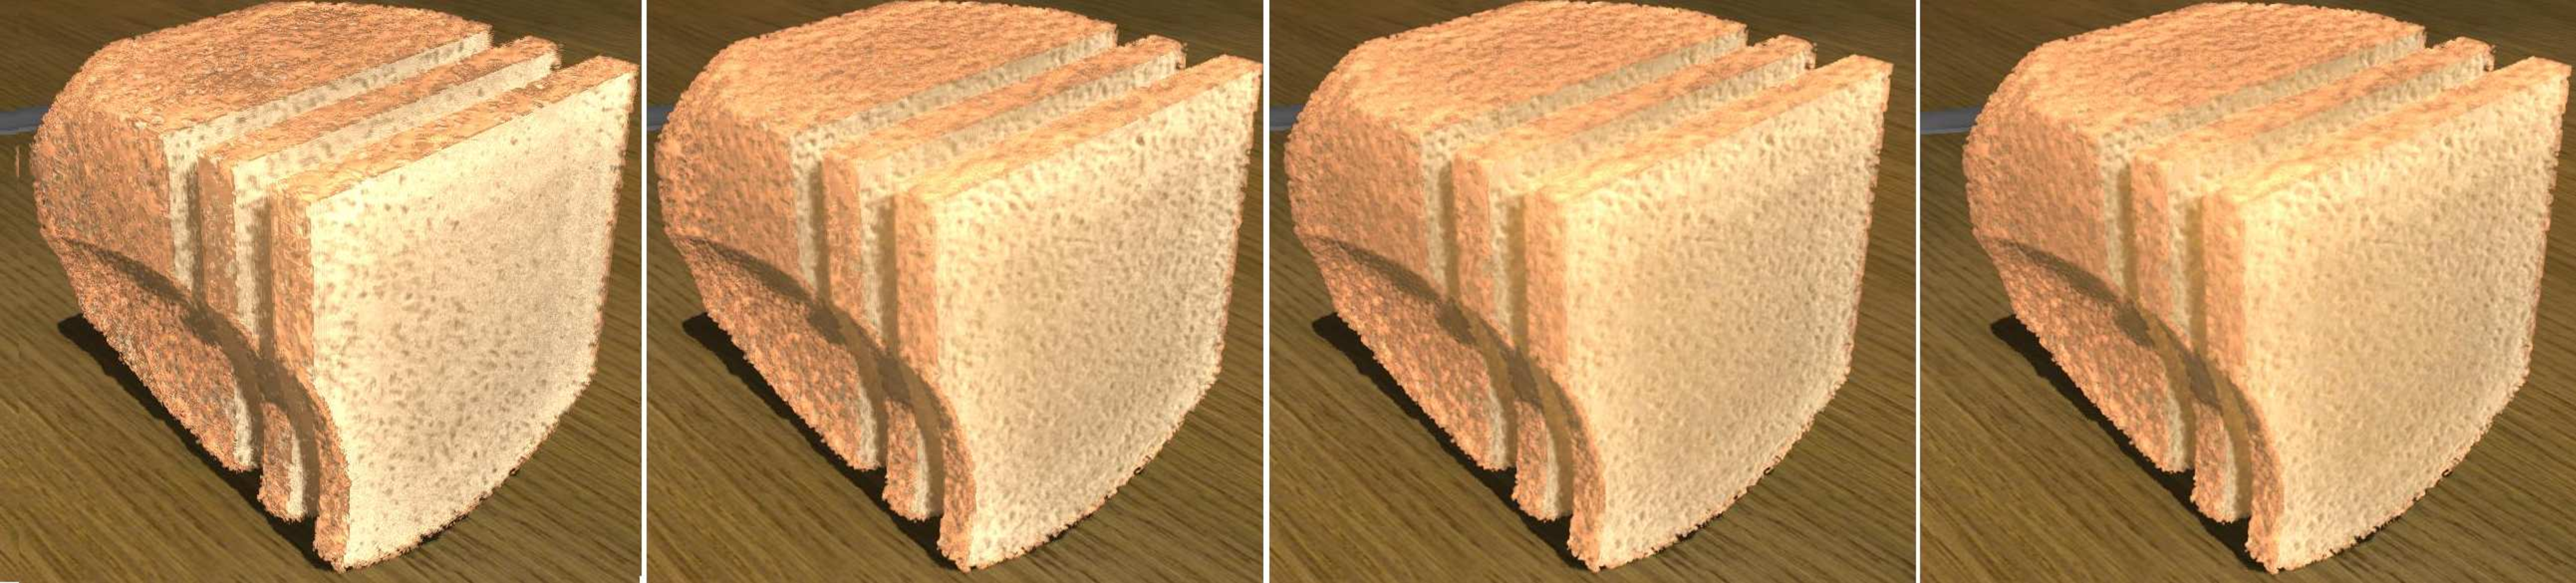
\includegraphics[width=12cm]{stepcount.pdf}

\begin{tabular}{|c|c|c|c|c|c|c|}
\hline
 Pasos del rayo         & 128 &  256 \\
\hline
\hline
 Tiempo total shaders   & 10 ms &  32.5 ms \\
\hline
 Rayo Principal         & 2 ms  & 5 ms  \\
\hline
 Rayos Secundarios      &  8 ms & 27.5 ms  \\
\hline
\end{tabular}
\caption{Detalle de tiempos de renderizado en milisegundos.}
\label{tab:n2}
\end{table}


\end{frame}

\begin{frame}{Renderizado utilizando más de una escala}
A la hora de obtener complejidad en la imagen resultante, existen limitaciones en la resolución de la textura.

Una solución consiste en utilizar más de una textura

\centerline{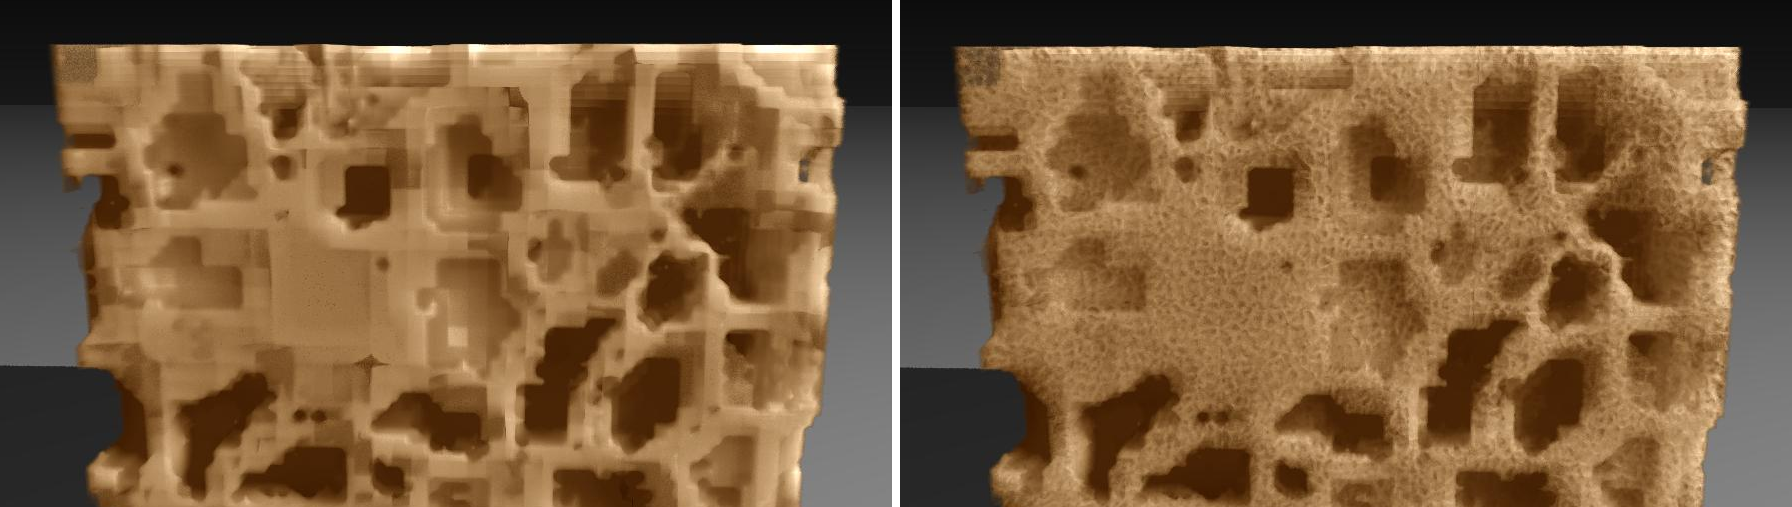
\includegraphics[width=10cm]{../figures/multiscale}}

Textura A muestreada en $(x,y,z)$

Textura B muestreada en $N\times (x,y,z), N \in \mathbb{R}$

\end{frame}



\begin{frame}{Conclusiones}
\begin{itemize}
\item Imágenes realistas
\item Tiempo real
\item Implementación simple
\end{itemize}

\begin{block}{Trabajos a Futuro}
\begin{itemize}
\item Otros materiales
\end{itemize}
\end{block}
\end{frame}

\section{Validación}



\begin{frame}
\begin{block}{}
\begin{center}
\vspace{1cm}
\huge{Validación}
\vspace{1cm}
\end{center}
\end{block}
\end{frame}


\subsection{Validación automática}

\begin{frame}{Validación automática}
Proponemos utilizar un \textbf{algoritmo}, en la validación de las geometrías porosas obtenidas, en oposición a una inspección subjetiva de los resultados.

En la generación utilizamos un algoritmo fractal para construir la geometría de migas de pan.

La estructura visible de la miga de pan sugiere que un algoritmo de extracción de características fractales podría describirla.


\end{frame}

\begin{frame}{Idea}
\begin{algorithm}[H]
\begin{algorithmic}[1]
\STATE Obtener espectro multifractal de muestras reales
\FOR{valores de parámetros}
\STATE Obtener espectro a partir de muestra sintética, generada con determinados valores de los parámetros
\STATE Comparar espectros reales con sintéticos
\ENDFOR
\STATE Devolver los parámetros más cercanos a los reales
\end{algorithmic}
\end{algorithm}
\end{frame}

\subsection{Fractales y Multifractales}

\begin{frame}{Dimensión Box}

\begin{wrapfigure}{r}{0.5\textwidth}
\includegraphics[width=6cm]{../figures/fitbox}
\end{wrapfigure}

Dada una imagen, se la subdividide en una grilla de dimensiones $M\times M$ donde el largo del lado de cada cuadrado formado es $\delta$. Si $N(\delta)$ representa el n\'umero de cuadrados que contienen al menos un p\'ixel resultado de una binarizaci\'on de la imagen (p\'ixel blanco) para ese $\delta$, la dimensi\'on Box $D_{b}$ queda definida como:\\

$$D_{b} = \displaystyle\lim_{\delta \to 0}{\frac{\log(N(\delta))}{\log (1/\delta)}}$$


\end{frame}

\begin{frame}
Esto sugiere que podría ser útil utilizar más de una DF para caracterizar los resultados.

El espectro multifractal puede ser utilizado para capturar distintas estructuras fractales dentro del mismo objeto, o distintos comportamientos fractales dependiendo de la escala.

La dimensión generalizada de orden $q$ con el método Sandbox se define como:

 \begin{align*}
D_{q\ne 1}^{sb} &= \frac{1}{q-1} \lim_{R \rightarrow 0}{
\frac{ln   { \left\langle  (M(R)/M_{0})^{q-1} \right\rangle   }}
{ln {(R/L)}       }},\\
D_{q=1}^{sb} &= \lim_{R \rightarrow 0}{
\frac{ \left\langle ln   { (M(R)/M_{0})  }  \right\rangle}
{ln {(R/L)}       }},
\end{align*}

\noindent donde $M_{0}$ es la cantidad de píxeles blancos en la imagen binarizada y $M(R)$ es el número de puntos que pertenecen a la estructura en un círculo de radio $R$ centrado en un punto de la misma.
\end{frame}

\begin{frame}
Se computó el espectro multifractal en muestras reales ({\em baguette} y pan casero), obteniendo las medianas de cada dimensión, con $q \in [-10,10]$.

Se compararon estos resultados con los sintéticos, por medio de la métrica de error:

\begin{equation*}
Error = \displaystyle \sum abs(medianas_{real}-medianas_{sint\acute{e}tico}).
\end{equation*}

Las imágenes sintéticas fueron generadas utilizando diversos parámetros en el leudado:

\begin{align*}
N &= \frac{k}{r^{d}},\\ r &= r_{min}+paso*j, j \in [0,\frac{r_{max}}{paso}],
\end{align*}
\noindent $k,d,r_{min},r_{max}$ y $step$ que controlan la generación de burbujas.

\end{frame}

\begin{frame}
\begin{figure}[!ht]
\includegraphics[width=7cm]{../figures/bestboxplot}
\caption[Mejores parámetros de síntesis para el tipo de pan {\em baguette}]{Mejores parámetros de síntesis para el tipo de pan {\em baguette}. El error total en medianas es de $\sim 0.21$.}
\label{bestboxplot}
\end{figure}

\end{frame}

\begin{frame}
\begin{figure}
\begin{center}
\includegraphics[width=6.5cm]{../figures/realbin}
\caption{ Pan {\em baguette} real y binarización.}
\label{realbin}
\end{center}
\end{figure}
Sintético:
\begin{center}
\includegraphics[width=3cm]{../figures/best}
\end{center}
\end{frame}


\begin{frame}
\begin{figure}
\includegraphics[width=7cm]{../figures/bestboxplot2}
\caption[Mejores parámetros de síntesis para un tipo casero de pan]{Mejores parámetros de síntesis para un tipo casero de pan. El error total en medianas es de $\sim 0.88$.}
\label{bestboxplot2}
\end{figure}

\end{frame}

\begin{frame}

\begin{figure}
\begin{center}
\includegraphics[width=7cm]{../figures/realbin2}
\caption{ Pan casero real y ejemplo de binarización.}
\label{realbin2}
\end{center}
\end{figure}

\begin{figure}
\begin{center}
\includegraphics[width=5cm]{../figures/best2}
\caption{Ejemplo de pan sintético con características similares a imágenes de un pan casero.}
\label{best2}
\end{center}
\end{figure}
\end{frame}



\begin{frame}{Conclusiones}
\begin{block}{}
\begin{itemize}
\item Algoritmo semi-automático para comparar muestras reales y sintéticas
\item Es posible utilizarlo para alimentar la generación a partir de una muestra real, y obtener un pan sintético con características estadísticamente similares.
\item Es posible mejorar el algoritmo hallando automáticamente los parámetros iniciales.
\end{itemize}
\end{block}

\end{frame}

\subsection{Extras}

\begin{frame}{Clasificación de Imágenes de cortes de Pan}
Adicionalmente se estudió el espectro multifractal para caracterizar y clasificar imágenes de cortes reales de pan.

Esto es útil para definir parámetros de calidad que deben respetar los panes reales, y proveer una clasificación automática de los mismos.

Se encontró que el MFS clasifica muestras de panes de manera comparable al estado del arte.

\end{frame}

\begin{frame}
\begin{table}[h!]
\center
% For LaTeX tables use
\begin{tabular}{lllllll}
\hline\noalign{\smallskip}
Método & Haralick & Lbp & SIFT & MFS & MFS CIELab\\ % & Zernicke
\noalign{\smallskip}\hline\noalign{\smallskip}
SVM & 94\% & 78.5\% & 96.5\% & 94.5\% & \textbf{97.5\%} \\
RF  & 91\% & 71.5\% & 92\% & 93.5\% & \textbf{96\%} \\
NN & 79\% & 70\% & 86\%  & 90.5\% & \textbf{92\%} \\
\noalign{\smallskip}\hline
\#FDs & 13 & 36 & 128 & 20 & 60\\
\hline
\end{tabular}
\caption{Resultados de la clasificación de migas de pan para diferentes características del estado del arte y diferentes algoritmos de clasificación.}
\label{tab:other} 
\end{table}
\end{frame}

\begin{frame}
Correlación entre las dimensiones del MFS y \\

\vspace{1cm}

\begin{tabular}{cc}
la fracción de vacío (VF) & el área media de las burbujas (MCA). \\
\includegraphics[width=5cm]{../figures/VF} & \includegraphics[width=5cm]{../figures/MCA} \\
\end{tabular}

\end{frame}

\begin{frame}
Correlación entre las dimensiones del MFS y el desvío estándar del área media de las burbujas (stCA)

\centerline{\includegraphics[width=5cm]{../figures/stMCA}}

\end{frame}

\begin{frame}{Conclusiones}
\begin{itemize}
\item Es posible utilizar el MFS no sólo para clasificar, sino para caracterizar muestras de panes.
\item Clasificación comparable al estado del arte.
\end{itemize}
\end{frame}


\begin{frame}{Validación utilizando Técnicas de Aprendizaje Profundo}
Recientemente se desarrollaron técnicas de Aprendizaje Profundo, los cuales clasifican una imagen entre miles de clases.

Los clasificadores se encuentran online, por lo cual es sencillo probar la clasificación con las imágenes generadas. Los resultados en panes son promisorios

\centerline{\includegraphics[width=5cm]{../figures/deep1}}

\end{frame}

\begin{frame}{Validación utilizando Técnicas de Aprendizaje Profundo}

\centerline{\includegraphics[width=4cm]{../figures/deep2}}
\centerline{\includegraphics[width=4cm]{../figures/deep3}}
\end{frame}
\begin{frame}{Validación utilizando Aprendizaje Profundo}
\centerline{\includegraphics[width=5cm]{../figures/deep4}}

\end{frame}



\section[Conclusiones]{Conclusiones y Trabajos a Futuro}


\begin{frame}
\begin{block}{}
\begin{center}
\vspace{1cm}
\huge{Conclusiones}
\vspace{1cm}
\end{center}
\end{block}
\end{frame}

\subsection{Conclusiones}
\begin{frame}{Conclusiones}
\begin{block}{}
\begin{itemize}
\item Se introdujo un algoritmo procedimental de generación de geometrías porosas.
\item Se presentó un algoritmo basado en el proceso real de formación del pan, eliminando decisiones ad-hoc en la generación de este material, obteniendo estructuras a lo largo de todo el proceso de formación.
\item Se aplicó un algoritmo de renderizado, basado en la interacción lumínica con una escena, produciendo imágenes foto-realísticas de materiales porosos/cocidos/comestibles como pan, esponjas, y piedras. Se obtuvieron imágenes \textbf{foto-realísticas} en tiempo real, por medio de la utilización de la GPU.
\end{itemize}
\end{block}
\end{frame}

\begin{frame}{Conclusiones}
\begin{block}{}
\begin{itemize}
\item Se validaron las geometrías generadas por el proceso inspirado en la formación del pan con muestras reales de pan.
\item Se presentó un método para clasificar muestras de pan, superando a clasificadores del estado del arte.
\end{itemize}
\end{block}
\end{frame}

\subsection{Trabajos a futuro}

\begin{frame}{Trabajos a futuro}
\begin{block}{}
\begin{itemize}
\item Generación procedimental de huesos y otros materiales
\item Validación tridimensional de los resultados
\item Validación utilizando técnicas de aprendizaje profundo
\item Implementación en GPU de la generación procedimental
\end{itemize}
\end{block}
\end{frame}

\begin{frame}
\centering

?`Preguntas?

\end{frame}

\begin{frame}
\centering

!`Gracias!

\end{frame}
\end{document}
